%%%%%%%%%%%%%%%%%%%%%%%%%%%%% Thesis.tex %%%%%%%%%%%%%%%%%%%%%%%%%%%%%%%
%                                                                      %
%  ---------- Master of Science Dissertation template ----------       %
%                                                                      %
%  Template for the Master Thesis according to the regulations         %
%  published by the Academic Board (Direcção Académica) at IST.        %
%                                                                      %
%  For up-to-date guide, please refer to the offical website           %
%  http://da.tecnico.ulisboa.pt/dissertacao-de-mestrado/               %
%                                                                      %
%       Andre C. Marta                                                 %
%       Area Cientifica de Mecanica Aplicada e Aeroespacial            %
%       Departamento de Engenharia Mecanica                            %
%       Instituto Superior Tecnico                                     %
%       Av. Rovisco Pais                                               %
%       1049-001 Lisboa                                                %
%       Portugal                                                       %
%       Tel: +351 21 841 9469                                          %
%                        3469 (extension)                              %
%       Email: andre.marta@tecnico.ulisboa.pt                          %
%                                                                      %
%  Created:       Jan 20, 2011                                         %
%  Last Modified: May  7, 2014                                         %
%                                                                      %
%%%%%%%%%%%%%%%%%%%%%%%%%%%%%%%%%%%%%%%%%%%%%%%%%%%%%%%%%%%%%%%%%%%%%%%%
%  Revision history                                                    %
%  v1 - 2011/01/24 - original template                                 %
%  v2 - 2012/10/30 - new IST image and glossary support                %
%  v3 - 2013/12/10 - update according to 2012/13 official guide        %
%  v4 - 2014/02/28 - new default for bibliography style                %
%  v5 - 2014/05/07 - update according to 2013/14 official guide        %
%%%%%%%%%%%%%%%%%%%%%%%%%%%%%%%%%%%%%%%%%%%%%%%%%%%%%%%%%%%%%%%%%%%%%%%%
%                                                                      %
% To generate the PDF file, type "make" at the terminal prompt.        %
%                                                                      %
% The IST template LaTeX package was created by the author             %
% and it can be downloaded from:                                       %
% https://fenix.ist.utl.pt/homepage/ist31052/                          %
%                                                                      %
% The external packages can be downloaded from                         %
% the Comprehensive TeX Archive Network at http://www.ctan.org/        %
%                                                                      %
% List of LaTex symbols:                                               %
% http://www.ctan.org/tex-archive/info/symbols/comprehensive/          %
%                                                                      %
% Help with LaTex can be found at                                      %
% http://www.giss.nasa.gov/tools/latex/ltx-2.html                      %
% http://en.wikibooks.org/wiki/LaTeX                                   %
%%%%%%%%%%%%%%%%%%%%%%%%%%%%%%%%%%%%%%%%%%%%%%%%%%%%%%%%%%%%%%%%%%%%%%%%

%%%%%%%%%%%%%%%%%%%%%%%%%%%%%%%%%%%%%%%%%%%%%%%%%%%%%%%%%%%%%%%%%%%%%%%%
%     Preamble                                                         %
%%%%%%%%%%%%%%%%%%%%%%%%%%%%%%%%%%%%%%%%%%%%%%%%%%%%%%%%%%%%%%%%%%%%%%%%

% ----------------------------------------------------------------------
%  Set the document class
% ----------------------------------------------------------------------
\documentclass[10pt,a4paper,twoside]{report}
\usepackage[export]{adjustbox}
% ----------------------------------------------------------------------
% Define external packages, language, margins, fonts and new commands
% change img folder in this file
% ----------------------------------------------------------------------
%%%%%%%%%%%%%%%%%%%%%%%%%%%%%%%%%%%%%%%%%%%%%%%%%%%%%%%%%%%%%%%%%%%%%%%%
%                                                                      %
%     File: Thesis_Preamble.tex                                        %
%     Tex Master: Thesis.tex                                           %
%                                                                      %
%     Author: Andre C. Marta                                           %
%     Last modified : 28 Feb 2014                                      %
%                                                                      %
%%%%%%%%%%%%%%%%%%%%%%%%%%%%%%%%%%%%%%%%%%%%%%%%%%%%%%%%%%%%%%%%%%%%%%%%

% ----------------------------------------------------------------------
% Define document language.
% ----------------------------------------------------------------------

% 'inputenc' package
%
% Accept different input encodings.
% http://www.ctan.org/tex-archive/macros/latex/base/
%
% > allows typing non-english text in LaTeX sources.
%
% ******************************* SELECT *******************************
%\usepackage[latin1]{inputenc} % <<<<< Windows
\usepackage[utf8]{inputenc}   % <<<<< Linux
% ******************************* SELECT *******************************



% 'babel' package
%
% Multilingual support for Plain TeX or LaTeX.
% http://www.ctan.org/tex-archive/macros/latex/required/babel/
%
% > sets the variable names according to the language selected
%
% ******************************* SELECT *******************************
%\usepackage[portuguese]{babel} % <<<<< Portuguese
\usepackage[english]{babel} % <<<<< English
% ******************************* SELECT *******************************


% List of LaTeX variable names: \abstractname, \appendixname, \bibname,
%   \chaptername, \contentsname, \listfigurename, \listtablename, ...)
% http://www.tex.ac.uk/cgi-bin/texfaq2html?label=fixnam
%
% Changing the words babel uses (uncomment and redefine as necessary...)
%
\newcommand{\acknowledgments}{@undefined} % new LaTeX variable name
%
% > English
%
\addto\captionsenglish{\renewcommand{\acknowledgments}{Acknowledgments}}
%\addto\captionsenglish{\renewcommand{\listtablename}{List of Tables}}
%\addto\captionsenglish{\renewcommand{\listfigurename}{List of Figures}}
%\addto\captionsenglish{\renewcommand{\nomname}{Nomenclature}}
%\addto\captionsenglish{\renewcommand{\glossaryname}{Glossary}}
%\addto\captionsenglish{\renewcommand{\acronymname}{List of Acronyms}}
%\addto\captionsenglish{\renewcommand{\bibname}{References}} % Bibliography
%\addto\captionsenglish{\renewcommand{\appendixname}{Appendix}}

% > Portuguese
%
\addto\captionsportuguese{\renewcommand{\acknowledgments}{Agradecimentos}}
%\addto\captionsportuguese{\renewcommand{\listtablename}{Lista de Figuras}}
%\addto\captionsportuguese{\renewcommand{\listfigurename}{Lista de Tabelas}}
\addto\captionsportuguese{\renewcommand{\nomname}{Lista de S\'{i}mbolos}} % Nomenclatura
%\addto\captionsportuguese{\renewcommand{\glossary}{Gloss\'{a}rio}}
%\addto\captionsportuguese{\renewcommand{\acronymname}{Lista de Abrevia\c{c}\~{o}es}}
%\addto\captionsportuguese{\renewcommand{\bibname}{Refer\^{e}ncias}} % Bibliografia
%\addto\captionsportuguese{\renewcommand{\appendixname}{Anexo}} % Apendice


% ----------------------------------------------------------------------
% Define default and cover page fonts.
% ----------------------------------------------------------------------

% Use Arial font as default
%
\renewcommand{\rmdefault}{phv}
\renewcommand{\sfdefault}{phv}

% Define cover page fonts
%
%         encoding     family       series      shape
%  \usefont{T1}     {phv}=helvetica  {b}=bold    {n}=normal
%                   {ptm}=times      {m}=normal  {sl}=slanted
%                                                {it}=italic
% see more examples at
% http://julien.coron.free.fr/languages/latex/fonts/
%
\def\FontLn{% 16 pt normal
  \usefont{T1}{phv}{m}{n}\fontsize{16pt}{16pt}\selectfont}
\def\FontLb{% 16 pt bold
  \usefont{T1}{phv}{b}{n}\fontsize{16pt}{16pt}\selectfont}
\def\FontMn{% 14 pt normal
  \usefont{T1}{phv}{m}{n}\fontsize{14pt}{14pt}\selectfont}
\def\FontMb{% 14 pt bold
  \usefont{T1}{phv}{b}{n}\fontsize{14pt}{14pt}\selectfont}
\def\FontSn{% 12 pt normal
  \usefont{T1}{phv}{m}{n}\fontsize{12pt}{12pt}\selectfont}


% ----------------------------------------------------------------------
% Define page margins and line spacing.
% ----------------------------------------------------------------------

% 'geometry' package
%
% Flexible and complete interface to document dimensions.
% http://www.ctan.org/tex-archive/macros/latex/contrib/geometry/
%
% > set the page margins (2.5cm minimum in every side, as per IST rules)
%
\usepackage{geometry}	
\geometry{verbose,tmargin=2.5cm,bmargin=2.5cm,lmargin=2.5cm,rmargin=2.5cm}

% 'setspace' package
%
% Set space between lines.
% http://www.ctan.org/tex-archive/macros/latex/contrib/setspace/
%
% > allow setting line spacing (line spacing of 1.5, as per IST rules)
%
\usepackage{setspace}
\renewcommand{\baselinestretch}{1.5}


% ----------------------------------------------------------------------
% Include external packages.
% Note that not all of these packages may be available on all system
% installations. If necessary, include the .sty files locally in
% the <jobname>.tex file directory.
% ----------------------------------------------------------------------

% 'graphicx' package
%
% Enhanced support for graphics.
% http://www.ctan.org/tex-archive/macros/latex/required/graphics/
%
% > extends arguments of the \includegraphics command
%
\usepackage{graphicx}

\graphicspath{{/home/chiroptera/workspace/thesis_writing/rsc/}}
% \DeclareGraphicsExtensions{.png,.eps}

% 'epstopdf' package
% Allows EPS images to be converted to PDF format.
%

 \usepackage{epstopdf}


% 'color' package
%
% Colour control for LaTeX documents.
% http://www.ctan.org/tex-archive/macros/latex/required/graphics/
%
% > defines color macros: \color{<color name>}
%
%\usepackage{color}


% 'amsmath' package
%
% Mathematical enhancements for LaTeX.
% http://www.ctan.org/tex-archive/macros/latex/required/amslatex/
%
% > American Mathematical Society plain Tex macros
%
\usepackage{amsmath}  % AMS mathematical facilities for LaTeX.
\usepackage{amsthm}   % Typesetting theorems (AMS style).
\usepackage{amsfonts} % 


% 'wrapfig' package
%
% Produces figures which text can flow around.
% http://www.ctan.org/tex-archive/macros/latex/contrib/wrapfig/
%
% > wrap figures/tables in text (i.e., Di Vinci style)
%
% \usepackage{wrapfig}


% 'subfigure' package
%
% Deprecated: Figures divided into subfigures.
% http://www.ctan.org/tex-archive/obsolete/macros/latex/contrib/subfigure/
%
% > subcaptions for subfigures
%
% \usepackage{subfigure}
\usepackage{caption}
\usepackage{subcaption}


% 'subfigmat' package
%
% Automates layout when using the subfigure package.
% http://www.ctan.org/tex-archive/macros/latex/contrib/subfigmat/
%
% > matrices of similar subfigures
%
% \usepackage{subfigmat}


% 'url' package
%
% Verbatim with URL-sensitive line breaks.
% http://www.ctan.org/tex-archive/macros/latex/contrib/url/
%
% > URLs in BibTex
%
% \usepackage{url}


% 'varioref' package
%
% Intelligent page references.
% http://www.ctan.org/tex-archive/macros/latex/required/tools/
%
% > smart page, figure, table and equation referencing
%
%\usepackage{varioref}


% 'dcolumn' package
%
% Align on the decimal point of numbers in tabular columns.
% http://www.ctan.org/tex-archive/macros/latex/required/tools/
%
% > decimal-aligned tabular math columns
%
\usepackage{dcolumn}
\newcolumntype{d}{D{.}{.}{-1}} % column aligned by the point separator '.'
\newcolumntype{e}{D{E}{E}{-1}} % column aligned by the exponent 'E'


% '' package
%
% Reimplementation of and extensions to LaTeX verbatim.
% http://www.ctan.org/tex-archive/macros/latex/required/tools/
%
% > provides the verbatim environment (\begin{verbatim},\end{verbatim})
%   and a comment environment (\begin{comment},  \end{comment})
%
% \usepackage{verbatim}


% 'moreverb' package
%
% Extended verbatim.
% http://www.ctan.org/tex-archive/macros/latex/contrib/moreverb/
%
% > supports tab expansion and line numbering
%
% \usepackage{moreverb}



% 'nomencl' package
%
% Produce lists of symbols as in nomenclature.
% http://www.ctan.org/tex-archive/macros/latex/contrib/nomencl/
%
% The nomencl package makes use of the MakeIndex program
% in order to produce the nomenclature list.
%
% Nomenclature
% 1) On running the file through LATEX, the command \makenomenclature
%    in the preamble instructs it to create/open the nomenclature file
%    <jobname>.nlo corresponding to the LATEX file <jobname>.tex and
%    writes the information from the \nomenclature commands to this file.
% 2) The next step is to invoke MakeIndex in order to produce the
%    <jobname>.nls file. This can be achieved by making use of the
%    command: makeindex <jobname>.nlo -s nomencl.ist -o <jobname>.nls
% 3) The last step is to invoke LATEX on the <jobname>.tex file once
%    more. There, the \printnomenclature in the document will input the
%    <jobname>.nls file and process it according to the given options.
%
% http://www-h.eng.cam.ac.uk/help/tpl/textprocessing/nomencl.pdf
%
% Nomenclature (produces *.nlo *.nls files)
\usepackage{nomencl}
\makenomenclature
%
% Group variables according to their symbol type
%
\RequirePackage{ifthen} 
\ifthenelse{\equal{\languagename}{english}}%
    { % English
    \renewcommand{\nomgroup}[1]{%
      \ifthenelse{\equal{#1}{R}}{%
        \item[\textbf{Roman symbols}]}{%
        \ifthenelse{\equal{#1}{G}}{%
          \item[\textbf{Greek symbols}]}{%
          \ifthenelse{\equal{#1}{S}}{%
            \item[\textbf{Subscripts}]}{%
            \ifthenelse{\equal{#1}{T}}{%
              \item[\textbf{Su
              perscripts}]}{}}}}}%
    }{% Portuguese
    \renewcommand{\nomgroup}[1]{%
      \ifthenelse{\equal{#1}{R}}{%
        \item[\textbf{Simbolos romanos}]}{%
        \ifthenelse{\equal{#1}{G}}{%
          \item[\textbf{Simbolos gregos}]}{%
          \ifthenelse{\equal{#1}{S}}{%
            \item[\textbf{Subscritos}]}{%
            \ifthenelse{\equal{#1}{T}}{%
              \item[\textbf{Sobrescritos}]}{}}}}}%
    }%


% 'glossary' package
%
% Create a glossary.
% http://www.ctan.org/tex-archive/macros/latex/contrib/glossary/
%
% Glossary (produces *.glo *.ist files)
\usepackage[number=none]{glossary}
% (remove blank line between groups)
\setglossary{gloskip={}}
% (redefine glossary style file)
%\renewcommand{\istfilename}{myGlossaryStyle.ist}
\makeglossary


% 'rotating' package
%
% Rotation tools, including rotated full-page floats.
% http://www.ctan.org/tex-archive/macros/latex/contrib/rotating/
%
% > show wide figures and tables in landscape format:
%   use \begin{sidewaystable} and \begin{sidewaysfigure}
%   instead of 'table' and 'figure', respectively.
%
\usepackage{rotating}


% 'algorithm' package
%
\usepackage{algorithm}
\usepackage[noend]{algpseudocode}
% \usepackage[options]{algorithm2e}
% \usepackage[]{algorithm2e}


% 'hyperref' package
%
% Extensive support for hypertext in LaTeX.
% http://www.ctan.org/tex-archive/macros/latex/contrib/hyperref/
%
% > Extends the functionality of all the LATEX cross-referencing
%   commands (including the table of contents, bibliographies etc) to
%   produce \special commands which a driver can turn into hypertext
%   links; Also provides new commands to allow the user to write adhoc
%   hypertext links, including those to external documents and URLs.
%
\usepackage[pdftex]{hyperref} % enhance documents that are to be
                              % output as HTML and PDF
\hypersetup{colorlinks,       % color text of links and anchors,
                              % eliminates borders around links
%            linkcolor=red,    % color for normal internal links
            linkcolor=black,  % color for normal internal links
            anchorcolor=black,% color for anchor text
%            citecolor=green,  % color for bibliographical citations
            citecolor=black,  % color for bibliographical citations
%            filecolor=magenta,% color for URLs which open local files
            filecolor=black,  % color for URLs which open local files
%            menucolor=red,    % color for Acrobat menu items
            menucolor=black,  % color for Acrobat menu items
%            pagecolor=red,    % color for links to other pages
            pagecolor=black,  % color for links to other pages
%            urlcolor=cyan,    % color for linked URLs
            urlcolor=black,   % color for linked URLs
	          bookmarks=true,         % create PDF bookmarks
	          bookmarksopen=false,    % don't expand bookmarks
	          bookmarksnumbered=true, % number bookmarks
	          pdftitle={Thesis},
            pdfauthor={Diogo Silva},
            pdfsubject={Efficient Evidence Accumulation Clustering for large datasets/big data},
            pdfkeywords={},
            pdfstartview=FitV,
            pdfdisplaydoctitle=true}


% 'hypcap' package
%
% Adjusting the anchors of captions.
% http://www.ctan.org/tex-archive/macros/latex/contrib/oberdiek/
%
% > fixes the problem with hyperref, that links to floats points
%   below the caption and not at the beginning of the float.
%
\usepackage[figure,table]{hypcap}

% 'booktabs' package
%
% nicer tables
%
\usepackage{booktabs}

% 'natbib' package
%
% Flexible bibliography support.
% http://www.ctan.org/tex-archive/macros/latex/contrib/natbib/
%
% > produce author-year style citations
%
% \citet  and \citep  for textual and parenthetical citations, respectively
% \citet* and \citep* that print the full author list, and not just the abbreviated one
% \citealt is the same as \citet but without parentheses. Similarly, \citealp is \citep without parentheses
% \citeauthor
% \citeyear
% \citeyearpar
%
% ******************************* SELECT *******************************
% \usepackage{natbib}          % <<<<< References in alphabetical list Correia, Silva, ...
\usepackage[numbers]{natbib} % <<<<< References in numbered list [1],[2],...
% ******************************* SELECT *******************************


% ----------------------------------------------------------------------
% Define new commands to assure consistent treatment throughout document
% ----------------------------------------------------------------------

\newcommand{\ud}{\mathrm{d}}                % total derivative
\newcommand{\degree}{\ensuremath{^\circ\,}} % degrees

% Abbreviations

\newcommand{\mcol}{\multicolumn}            % table format

\newcommand{\eqnref}[1]{(\ref{#1})}
\newcommand{\class}[1]{\texttt{#1}}
\newcommand{\package}[1]{\texttt{#1}}
\newcommand{\file}[1]{\texttt{#1}}
\newcommand{\BibTeX}{\textsc{Bib}\TeX}

% Typefaces ( example: {\bf Bold text here} )
%
% > pre-defined
%   \bf % bold face
%   \it % italic
%   \tt % typewriter
%
% > newly defined
\newcommand{\tr}[1]{{\ensuremath{\textrm{#1}}}}   % text roman
\newcommand{\tb}[1]{{\ensuremath{\textbf{#1}}}}   % text bold face
\newcommand{\ti}[1]{{\ensuremath{\textit{#1}}}}   % text italic
\newcommand{\mc}[1]{{\ensuremath{\mathcal{#1}}}}  % math calygraphy
\newcommand{\mco}[1]{{\ensuremath{\mathcalold{#1}}}}% math old calygraphy
\newcommand{\mr}[1]{{\ensuremath{\mathrm{#1}}}}   % math roman
\newcommand{\mb}[1]{{\ensuremath{\mathbf{#1}}}}   % math bold face
\newcommand{\bs}[1]{\ensuremath{\boldsymbol{#1}}} % math symbol
\def\bm#1{\mathchoice                             % math bold
  {\mbox{\boldmath$\displaystyle#1$}}%
  {\mbox{\boldmath$#1$}}%
  {\mbox{\boldmath$\scriptstyle#1$}}%
  {\mbox{\boldmath$\scriptscriptstyle#1$}}}
\newcommand{\boldcal}[1]{{\ensuremath{\boldsymbol{\mathcal{#1}}}}}% math bold calygraphy



% \usepackage{tablefootnote}
\usepackage{longtable}


\newcommand{\rscpath}{/home/chiroptera/workspace/thesis_writing/rsc}

\usepackage{csquotes}
%\usepackage[doi=false]{biblatex}%style=numeric-comp,
 % file "Thesis_Preamble.tex"


%%%%%%%%%%%%%%%%%%%%%%%%%%%%%%%%%%%%%%%%%%%%%%%%%%%%%%%%%%%%%%%%%%%%%%%%
%     Begin Document                                                   %
%%%%%%%%%%%%%%%%%%%%%%%%%%%%%%%%%%%%%%%%%%%%%%%%%%%%%%%%%%%%%%%%%%%%%%%%
\begin{document}

% Set plain page style (no headers, footer with centered page number)
\pagestyle{plain}

% Set roman numbering (i,ii,...) before the start of chapters
\pagenumbering{roman}

% ----------------------------------------------------------------------
%  Cover page
% ----------------------------------------------------------------------
%%%%%%%%%%%%%%%%%%%%%%%%%%%%%%%%%%%%%%%%%%%%%%%%%%%%%%%%%%%%%%%%%%%%%%%%
%                                                                      %
%     File: Thesis_FrontCover.tex                                      %
%     Tex Master: Thesis.tex                                           %
%                                                                      %
%     Author: Andre C. Marta                                           %
%     Last modified :  7 May 2014                                      %
%                                                                      %
%%%%%%%%%%%%%%%%%%%%%%%%%%%%%%%%%%%%%%%%%%%%%%%%%%%%%%%%%%%%%%%%%%%%%%%%

\thispagestyle {empty}

% IST Logo - Signature A
% parameters: bb=llx lly urx ury (bounding box), width=h_length, height=v_length, angle=angle, scale=factor, clip=true/false, draft=true/false. 

\includegraphics[bb=9.5cm 15cm 0cm 0cm,scale=0.15]{Figures/afa}

\includegraphics[bb=-35cm 11cm 0cm 0cm,scale=0.29]{IST_A_CMYK_POS}



% 
\includegraphics[scale=0.29, right]{IST_A_CMYK_POS}
% 
\includegraphics[scale=0.15, left]{Figures/afa}

\begin{center}
%
% Figure (Image or plot)
\vspace{2.5cm}
% height = 50 mm
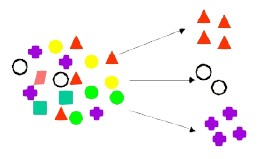
\includegraphics[height=50mm]{Figures/clustering.jpg}

% Title, author and degree
\vspace{1.0cm}
{\FontLb Efficient Evidence Accumulation Clustering for large datasets/big data} \\
%\vspace{0.2cm}
%{\FontMn Subtitle (optional)} \\
%\vspace{1.9cm}
\vspace{2.7cm}
{\FontMb Diogo Alexandre Oliveira Silva} \\
\vspace{2.0cm}
{\FontSn Thesis to obtain the Master of Science Degree in} \\
\vspace{0.3cm}
% {\FontLb Electrical and Computer Engineering} \\
{\FontLb Aeronautical Military Sciences in the speciality of Electrical Engineering} \\
\vspace{1.1cm}
% {\FontSn Supervisors: Dra. Ana Fred and Dra. Helena Aidos} \\
\vspace{1.1cm}
{\FontMb Examination Committee} \\
\vspace{0.3cm}
{\FontSn %
\begin{tabular}{ll}
Chairperson: & Professor Full Name \\
Supervisor: & Dra. Ana Luísa Nobre Fred \\
Co-supervisor: & Dra. Helena Aidos Lopes \\
Member of the Committee: & Professor Full Name 3
\end{tabular} } \\
\vspace{1.5cm}
{\FontMb Month 2015} \\
%
\end{center}

\cleardoublepage

 % file "Thesis_FrontCover.tex"

% ----------------------------------------------------------------------
% Dedication page (optional)
% ----------------------------------------------------------------------
%%%%%%%%%%%%%%%%%%%%%%%%%%%%%%%%%%%%%%%%%%%%%%%%%%%%%%%%%%%%%%%%%%%%%%%%
%                                                                      %
%     File: Thesis_Dedication.tex                                      %
%     Tex Master: Thesis.tex                                           %
%                                                                      %
%     Author: Andre C. Marta                                           %
%     Last modified : 21 Jan 2011                                      %
%                                                                      %
%%%%%%%%%%%%%%%%%%%%%%%%%%%%%%%%%%%%%%%%%%%%%%%%%%%%%%%%%%%%%%%%%%%%%%%%

\null\vskip5cm%
\begin{flushright}
     Dedicated to someone special...
\end{flushright}
\vfill\newpage

\cleardoublepage

 % file "Thesis_Dedication.tex"

% ----------------------------------------------------------------------
%  Acknowledgments (optional)
% ----------------------------------------------------------------------
%%%%%%%%%%%%%%%%%%%%%%%%%%%%%%%%%%%%%%%%%%%%%%%%%%%%%%%%%%%%%%%%%%%%%%%%
%                                                                      %
%     File: Thesis_Acknowledgments.tex                                 %
%     Tex Master: Thesis.tex                                           %
%                                                                      %
%     Author: Andre C. Marta                                           %
%     Last modified : 21 Jan 2011                                      %
%                                                                      %
%%%%%%%%%%%%%%%%%%%%%%%%%%%%%%%%%%%%%%%%%%%%%%%%%%%%%%%%%%%%%%%%%%%%%%%%

\section*{\acknowledgments}

% Add entry in the table of contents as section
\addcontentsline{toc}{section}{\acknowledgments}

%Supervisors
It would come as a great oversight if I was not aware of the help and contribution I received for the completion of this undertaking.

I should start by expressing deep appreciation to my supervisors, Dr. Ana Fred and Dr. Helena Lopes.
The freedom I was allowed was crucial for keeping my motivation up for such a long period.
When that was lacking, their guidance and encouragement quickly put me back on track.

%Family & Friends
I leave my warmest regards to the family I built throughout my military and academic career, during these last years.
Your camaraderie has shaped where I stand and who I am today.
Your support throughout these long months was invaluable.

% Bella
To my loving girlfriend, who would always hear my boundless enthusiasm or disheartening frustrations, whichever was the case, and who followed me closest in the last months, I am deeply grateful.
You motivated me most of all, and that was no small task.

And to my parents, thank you for all your support and motivation during all these years.
You were always caring and encouraging and I am forever grateful for that.

Last, but not least, thank you to all my friends and family for understanding my absence during these challenging months.
\cleardoublepage

 % file "Thesis_Acknowledgements.tex"

% ----------------------------------------------------------------------
%  Abstract (both in English and Portuguese)
% ----------------------------------------------------------------------
%%%%%%%%%%%%%%%%%%%%%%%%%%%%%%%%%%%%%%%%%%%%%%%%%%%%%%%%%%%%%%%%%%%%%%%%
%                                                                      %
%     File: Thesis_Resumo.tex                                          %
%     Tex Master: Thesis.tex                                           %
%                                                                      %
%     Author: Andre C. Marta                                           %
%     Last modified : 21 Jan 2011                                      %
%                                                                      %
%%%%%%%%%%%%%%%%%%%%%%%%%%%%%%%%%%%%%%%%%%%%%%%%%%%%%%%%%%%%%%%%%%%%%%%%

\section*{Resumo}

% Add entry in the table of contents as section
\addcontentsline{toc}{section}{Resumo}

Avanços na tecnologia permitem a recolha e armazenamento de quantidades e variedades de dados sem precedente.
A maior parte destes dados são armazenados eletrónicamente e existe interesse em realizar análise automática dos mesmos.
As técnicas de \emph{clustering} estão entre as mais populares para essa tarefa porque não assumem nada sobre a estrutura dos dados \emph{a priori}.
Dezenas de técnicas existem, mas, típicamente, uma só técnica não tem um bom desempenho em todos os conjuntos de dados devido às especifidades de cada um.
Técnicas de \emph{ensemble clustering} tentam responder a esse desafio ao combinar outros algoritmos.
Esta dissertação foca-se numa em particular, o \emph{Evidence Accumulation Clustering} (EAC).
O EAC é uma algorithm robusto que tem demonstrado bons desempenhos na literatura numa variedade de conjuntos de dados.
No entanto, esta robustez vem com um maior custo computacional associado.
A sua aplicação não só é mais lenta como está restrita a conjuntos de dados pequenos.
Assim, o objetivo desta dissertação é escalar o EAC, possibilitando a sua a aplicação a conjuntos de dados grandes (mais que $500 \: 000$ amostras), com tecnologia disponivel numa típica estação de trabalho.
Com isto em mente, várias abordagens foram exploradas: acelerar processamento com outros algoritmos (\emph{quantum clustering}), através de processamento paralelo (com GPU), escalar para maiores conjuntos de dados com algoritmos de memória externa (disco rígido) e explorando a natureza esparsa do EAC.
Uma contribuição de relevo é um método novo para construir uma matriz de esparsa específico ao EAC.
Os resultados mostram que a solução proposta é, efetivamente, aplicável a conjuntos de dados grandes e é significativamente mais rápida que a original para conjuntos pequenos.

\textbf{\Large Palavras-chave:} clustering, EAC, quantum clustering, K-Means, Single-Link, matriz esparsa, GPGPU





\cleardoublepage

 % file "Thesis_Resumo.tex"
%%%%%%%%%%%%%%%%%%%%%%%%%%%%%%%%%%%%%%%%%%%%%%%%%%%%%%%%%%%%%%%%%%%%%%%%
%                                                                      %
%     File: Thesis_Abstract.tex                                        %
%     Tex Master: Thesis.tex                                           %
%                                                                      %
%     Author: Andre C. Marta                                           %
%     Last modified : 21 Jan 2011                                      %
%                                                                      %
%%%%%%%%%%%%%%%%%%%%%%%%%%%%%%%%%%%%%%%%%%%%%%%%%%%%%%%%%%%%%%%%%%%%%%%%

\section*{Abstract}

% Add entry in the table of contents as section
\addcontentsline{toc}{section}{Abstract}

Advances in technology allow for the collection and storage of an unprecedent amount and variety of data.
Most of this data is stored electronically and there is an interest in automated analysis for generation of knowledge and new insights.
Since the structure of the data is unknown, clustering techniques become particularly interesting for knowledge discovery and data mining, as they make as few assumptions on the data as possible.
A vast body of work on these algorithms exist, yet, typically, no single algorithm is able to respond to the specificities of all data.
Ensemble clustering algorithm address this problem by combining other algorithms.
Evidence Accumulation Clustering (EAC) is a robust ensemble algorithm that has shown good results and is the focus of this dissertation.
However, this robustness comes with higher computational cost.
Its application is slower and restricted to smaller datasets.
Thus, the objective of this dissertation is to scale EAC, allowing its applicability to big datasets, with technology available at a typical workstation.
Accordingly, several approaches were explored: speed-up with other algorithms (\emph{quantum clustering}) or parallel computing (with GPU) and reducing space complexity by using external memory (hard drive) algorithms and exploiting the sparse nature of EAC.
A relevant contribution is a novel method to build a sparse matrix specialized in EAC.
Results show that the proposed solution is applicable to large datasets and presents speed-ups between 6 and 200 over the original implementation on different phases of EAC for small datasets.

\vfill

\textbf{\Large Key words:} Clustering methods, EAC, K-Means, MST, GPGPU, CUDA, Sparse matrices, Single-Link

\cleardoublepage

 % file "Thesis_Abstract.tex"

% ----------------------------------------------------------------------
%  Table of contents, list of tables, list of figures and nomenclature
% ----------------------------------------------------------------------

% Table of contents
%
\tableofcontents
\cleardoublepage 

% List of tables
%
% Generate list
\listoftables
% Add entry in the table of contents as section
\addcontentsline{toc}{section}{\listtablename}
\cleardoublepage 

% List of figures
%
% Generate list
\listoffigures
% Add entry in the table of contents as section
\addcontentsline{toc}{section}{\listfigurename}
\cleardoublepage 

% Nomenclature
%
% entries of nomenclature list
%%%%%%%%%%%%%%%%%%%%%%%%%%%%%%%%%%%%%%%%%%%%%%%%%%%%%%%%%%%%%%%%%%%%%%%%%
%                                                                      %
%     File: Thesis_Nomenclature.tex                                    %
%     Tex Master: Thesis.tex                                           %
%                                                                      %
%     Author: Andre C. Marta                                           %
%     Last modified : 21 Jan 2011                                      %
%                                                                      %
%%%%%%%%%%%%%%%%%%%%%%%%%%%%%%%%%%%%%%%%%%%%%%%%%%%%%%%%%%%%%%%%%%%%%%%%
%
% The definitions can be placed anywhere in the document body
% and their order is sorted by <symbol> automatically when
% calling makeindex in the makefile
%
% The \glossary command has the following syntax:
%
% \glossary{entry}
%
% The \nomenclature command has the following syntax:
%
% \nomenclature[<prefix>]{<symbol>}{<description>}
%
% where <prefix> is used for fine tuning the sort order,
% <symbol> is the symbol to be described, and <description> is
% the actual description.

% ----------------------------------------------------------------------
% Roman symbols [r]
\nomenclature[ru]{$\bf u$}{Velocity vector.}
\nomenclature[ru]{$u,v,w$}{Velocity Cartesian components.}
\nomenclature[rp]{$p$}{Pressure.}
\nomenclature[rC]{$C_D$}{Coefficient of drag.}
\nomenclature[rC]{$C_L$}{Coefficient of lift.}
\nomenclature[rC]{$C_M$}{Coefficient of moment.}

% ----------------------------------------------------------------------
% Greek symbols [g]
\nomenclature[g]{$\rho$}{Density.}
\nomenclature[g]{$\alpha$}{Angle of attack.}
\nomenclature[g]{$\beta$}{Angle of side-slip.}
\nomenclature[g]{$\mu$}{Molecular viscosity coefficient.}
\nomenclature[g]{$\kappa$}{Thermal conductivity coefficient.}

% ----------------------------------------------------------------------
% Subscripts [s]
\nomenclature[s]{$x,y,z$}{Cartesian components.}
\nomenclature[s]{$i,j,k$}{Computational indexes.}
\nomenclature[s]{$\infty$}{Free-stream condition.}
\nomenclature[s]{ref}{Reference condition.}
\nomenclature[s]{$n$}{Normal component.}

% ----------------------------------------------------------------------
% Supercripts [t]
\nomenclature[t]{T}{Transpose.}
\nomenclature[t]{*}{Adjoint.}

 % file "Thesis_Nomenclature.tex"
%
% Insert glossary/nomenclature section produced by MakeIndex
%\printnomenclature
% Add entry in the table of contents as section
%\addcontentsline{toc}{section}{\nomname}
%\cleardoublepage

% entries of glossary list
%%%%%%%%%%%%%%%%%%%%%%%%%%%%%%%%%%%%%%%%%%%%%%%%%%%%%%%%%%%%%%%%%%%%%%%%
%                                                                      %
%     File: Thesis_Glossary.tex                                        %
%     Tex Master: Thesis.tex                                           %
%                                                                      %
%     Author: Andre C. Marta                                           %
%     Last modified : 30 Oct 2012                                      %
%                                                                      %
%%%%%%%%%%%%%%%%%%%%%%%%%%%%%%%%%%%%%%%%%%%%%%%%%%%%%%%%%%%%%%%%%%%%%%%%
%
% The definitions can be placed anywhere in the document body
% and their order is sorted by <symbol> automatically when
% calling makeindex in the makefile
%
% The \glossary command has the following syntax:
%
% \glossary{entry}
%
% The \nomenclature command has the following syntax:
%
% \nomenclature[<prefix>]{<symbol>}{<description>}
%
% where <prefix> is used for fine tuning the sort order,
% <symbol> is the symbol to be described, and <description> is
% the actual description.

% ----------------------------------------------------------------------

\glossary{name={\textbf{MDO}},description={Multi-Disciplinar Optimization is an engineering technique that uses optimization methods to solve design problems incorporating two or more disciplines.}}

\glossary{name={\textbf{CFD}},description={Computational Fluid Dynamics is a branch of fluid mechanics that uses numerical methods and algorithms to solve problems that involve fluid flows.}}

\glossary{name={\textbf{CSM}},description={Computational Structural Mechanics is a branch of structure mechanics that uses numerical methods and algorithms to perform the analysis of structures and its components.}}

 % file "Thesis_Glossary.tex"

% Insert glossary section produced by MakeIndex
\printglossary
% Add entry in the table of contents as section
\addcontentsline{toc}{section}{\glossaryname}
\cleardoublepage

% Set arabic numbering (1,2,...) after preface
%
\setcounter{page}{1}
\pagenumbering{arabic}

% ----------------------------------------------------------------------
%  Chapters
% ----------------------------------------------------------------------

\chapter{Introduction}
\label{chapter:introduction}

%TODO (extra introduction)
% problems under Big Data paradihm
% typical challenges with Big Data
% why EAC?
% combination of both

\section{Challenges and Motivation}

% Estrutura mais clara:
% Motivacao: analise atomatica de dados numa perspectiva de
% analise exploratoria; exemplos; novos desafios face a grande
% quantidade de dados; tecnicas de clustering como as tecnicas
% formais de abordar estes problemas; dificuldades tradicionais
% que levaram ao state-of-art dos metodos de ensemble.
% Dificuldades adicionais asociados ao Big Data; face a isto a
% tese propoe abordar este problema ....
 
% Se quizeres, formulacao mais detalhada do problema com um
% exemplo mais motivador com dados reais: clustering, EAC, ...



% Motivacao: analise atomatica de dados numa perspectiva de
% analise exploratoria;
Advances in technology allow for the collection and storage of unprecedented amount and variety of data, a concept commonly designated by \emph{Big Data}.
Most of this data is stored electronically and there is an interest in automated analysis for generation of knowledge and new insights.
%examples of applications; jet engine example is nice for Air Force: taken from http://wikibon.org/wiki/v/Big_Data_in_the_Aviation_Industry; related Carnegie Mellon: http://bigdatasymposium.dsigroup.org/wp-content/uploads/2011/12/Dubrawski-DSI-Big-Data-Symposium-January-29-2013.pdf
The applications of such analysis are abundant and across many fields, ranging from recommender systems and customer segmentation in business, to predicting when a jet engine is likely to fail using sensor data, or even the study of gene expression in biomedics, to namy a few.

% examples of analisis tools
A growing body of statistical methods aiming to model, structure and/or classify data already exist, e.g. linear regression, principal component analysis, cluster analysis, support vector machines, neural networks.
% tecnicas de clustering como as tecnicas formais de abordar estes problemas
Cluster analysis is an interesting tool because it typically does not make assumptions on the structure of the data.
Since, often, the structure of the data is unknown, clustering techniques become particularly interesting for transforming this data into knowledge and discovering its underlying structure and patterns.
%Clustering is a ill defined problem, one of the reasons why there are hundreds of algorithms. 
Clustering is a hard problem and a vast body of work on these algorithms exist.
Yet, typically, no single algorithm is able to respond to the specificities of all data.
Different methods are suited to datasets of different characteristics and, often, the challenge of the researcher is to find the right algorithm for the task. %TODO get ref for this

% dificuldades tradicionais que levaram ao state-of-art dos metodos de ensemble.
Currently, there are state of the art algorithms that are more robust than "traditional" algorithms by having a wider applicability or being less dependent on input parameters, e.g. algorithms that do not take any parameters for performing an analysis.
One such algorithm is Evidence Accumulation Clustering (EAC), belonging to the wider class of ensemble methods.
EAC is a state-of-the art clustering algorithm that addresses the robustness challenge.
% novos desafios face a grande quantidade de dados; % Dificuldades adicionais asociados ao Big Data
However, the current reality of capturing massive amounts of data rises new challenges.
Two important challenges are efficiency and scalability, which translate on how fast the algorithms are and how well they scale when the input data multiplies in size, dimensionality and variety.
The algorithms themselves are no longer the only focus of research.
Much effort is being put into the scalability and performance of algorithms, which usually translates in addressing their computational complexity with parallelized computation and distributed memory being some of the proposed solutions.
Cluster analysis with EAC should be fast and able to scale to larger datasets as well as robust, so as to address the reality of big data.

%TODO review paragraph; it is a collection of phrases right now
% This sprouted the rise of new uses of existing computing architectures (e.g. Graphic Processing Units) and development of new programming models (e.g. Hadoop, shared and distributed memory).
% Each of these has its own specificities and the researcher must have an in-depth knowledge of the architectures and models used to frame the problems and obtain results.

% face a isto a tese propoe abordar este problema
This dissertation is concerned with pushing the current limits of the EAC to large datasets by addressing the problems of scalability and efficiency without compromising robustness, using technology available in a desktop workstation.
Processing of huge amounts of data has been out of the range of capability of the traditional desktop workstation.
This sprouted the rise of new uses of existing computing architectures (e.g. Graphic Processing Units) and development of new programming models (e.g. Hadoop, shared and distributed memory).
The problem at hand is, then, to  optimize the algorithm regarding both speed and memory usage.
This, of course, comes with challenges.
How can one keep the original accuracy while significantly increase efficiency?
Is there an exploitable trade-off between the three main characteristics: speed, memory and accuracy?
These are guiding questions that this dissertation addresses.


\section{Goals}

This dissertation aims to research and extend the state of the art of ensemble clustering, in what concerns the EAC method and its application to large datasets, while also assessing algorithmic solutions and parallelization techniques.
The goal is to understand EAC's suitability for large datasets and find ways to respond to the stated challenges, in terms of speed and memory.
The main objectives for this work are:

\begin{itemize}

\item Study the integration of quantum inspired methods in EAC.

\item Study the integration of the General Purpose computing in a Graphics Processing Unit (GPGPU) paradigm in EAC.

\item Devise strategies to reduce computation and memory complexities of EAC.

\item Application of Evidence Accumulation Clustering to Big Data.

\item Validation of Big Data EAC on real data.% (ECG for emotional state discovery and/or discovery of natural groups, or other datasets)
\end{itemize}

\section{Contributions}
The main contributions are the adaptation of the three distinct stages of the EAC framework to larger datasets.
In particular, an efficient parallel version for Graphics Processing Units (GPU) of the K-Means clustering algorithm is implemented for the first stage of EAC.
Still in this stage, two clustering algorithms in the young field of Quantum Clustering were reviewed, tested and evaluated having EAC in mind. % QK-Means and Horn
Different methods for the second stage were tested, using complete matrices and sparse matrices.% and a k-Nearest Neighbors scheme.
Worthy of mention is a novel and specialized method for building a sparse matrix in the second stage. % EAC CSR
%A post-processing operation on the second stage product was briefly studied. % the threshold cut
A GPU parallel version of a MST (Minimum Spanning Tree) solver algorithm was reviewed and tested for the last stage, a co-product of which was an algorithm to find the connected components of a MST.
A hard disk solution was implemented for dealing with large datasets whose space complexity in the final stage exceeded the available memory.


% Explain briefly the work done

% The scope of the thesis is Big Data and Cluster Ensembles.
% A main requirement in this context is to have fast clustering techniques.
% This may be accomplished in two ways: algorithmically or with parallelization techniques.
% The former deals with finding faster solutions while the latter takes existing solutions and optimizes them with execution speed in mind.

% The initial research was under the algorithmic path.
% More specifically, exploring quantum inspired clustering algorithms.
% The findings of this exploration revealed this algorithms to be a poor match for integration in EAC and turned the focus of the research to parallelization techniques.
% Two main paradigms of parallelization were found appropriate: GPGPU and distributed (among a cluster of workstations).
% While the first is a readily available resource in common machines, the second is able to address problems dealing with larger datasets.

\section{Outline}

Chapter \ref{chapter:clustering} provides an introduction to clustering nomenclature and concepts, as well as some "traditional" clustering algorithms.
Chapter \ref{chapter:stateofart} starts by reviewing the Evidence Accumulation Clustering algorithm in detail.
It goes on to review possible approaches to the problem of scaling EAC.
Based on an algorithmic approach, a review of the young field of quantum clustering is presented, with a more in-depth emphasis on two algorithms.
With a parallelization approach in mind, a programming model for the GPU (CUDA) is reviewed, followed by some parallelized versions of relevant algorithms to the problem of this dissertation.
The following chapter, \ref{chapter:methodology}, presents the approach that was actually taken to scale EAC.
It presents the steps taken on each part of the algorithm, the underlying difficulties and what was done to address them.
It also includes the reference of approaches that were developed but were not deemed suited to integrate the EAC toolchain.
In the results chapter, \ref{chapter:results}, the results of the different approaches of optimizing the EAC method are presented.
Chapter \ref{chapter:discussion} presents an interpretation and critical discussion of those results.
Finally, chapter \ref{chapter:conclusions} concludes the dissertation.
It also offers recommendations for future work. % file "Thesis_Introduction.tex"
%!TEX root = Thesis.tex

\chapter{Clustering}


\section{The problem of clustering}
\label{sec:clustering}

%this is mostly taken from Jain's 50 years beyond K-Means
Advances in technology allow for the collection and storage unprecedented amount and variety of data.
Since data is mostly stored electronically, it presents a potential for automatic analysis and thus creation of information and knowledge.
A growing body of statistical methods aiming to model, structure and/or classify data already exist, e.g. linear regression, principal component analysis, cluster analysis, support vector machines, neural networks.
Many of these methods fall into the realm of machine learning, which is usually divided into 2 major groups: \textit{supervised} and \textit{unsupervised} learning.
% TODO: add some reference for the 2 major groups; optional: explain what learning is
Supervised learning deals with labeled data, i.e. data for which ground truth is known, and tries to solve the problem of classification. %TODO: add ref for solving classification
Unsupervised learning deals with unlabeled data and tries to solve the problem of clustering. % TODO: add ref for solving clustering

Cluster analysis is the backbone of the present work.
The goal of data clustering, as defined by \cite{Jain2010}, is the discovery of the \textit{natural grouping(s)} of a set of patterns, points or objects.
In other words, the goal of data clustering is to discover structure on data.
And the methodology used is to group patterns that are similar by some metric (e.g. euclidean distance, Pearson correlation) and separate those that are dissimilar. %TODO reference for a method for both euclidean distance and Pearson correlation

As an example, Figure \ref{fig:intro raw} shows the plot of a simple synthetic dataset - a Gaussian mixture of 5 distributions.
No extra information other than the position of the points is given, since clustering algorithms are unsupervised methods.
Figure \ref{fig:intro natural} presents the desired (or "natural") clustering for this given dataset.
Figure \ref{fig:intro kmeans} presents the clusters given by the K-Means algorithm with an initialization of 4 clusters.
The number of clusters was purposefully set to an "incorrect" number to demonstrate that the number of cluster of a dataset is not trivial to discover, even in such a simple example.
In this synthetic dataset, the number of clusters is not clear due to the two superimposed Gaussians.
The number of clusters is a common initialization parameter for clustering methods.
When no prior information about the dataset is given, the number of clusters can be hard to discover.

%TODO change this 3 plots to a three plot subfigure, with the plots side by side
% \begin{figure}[hbtp]
% \centering
% 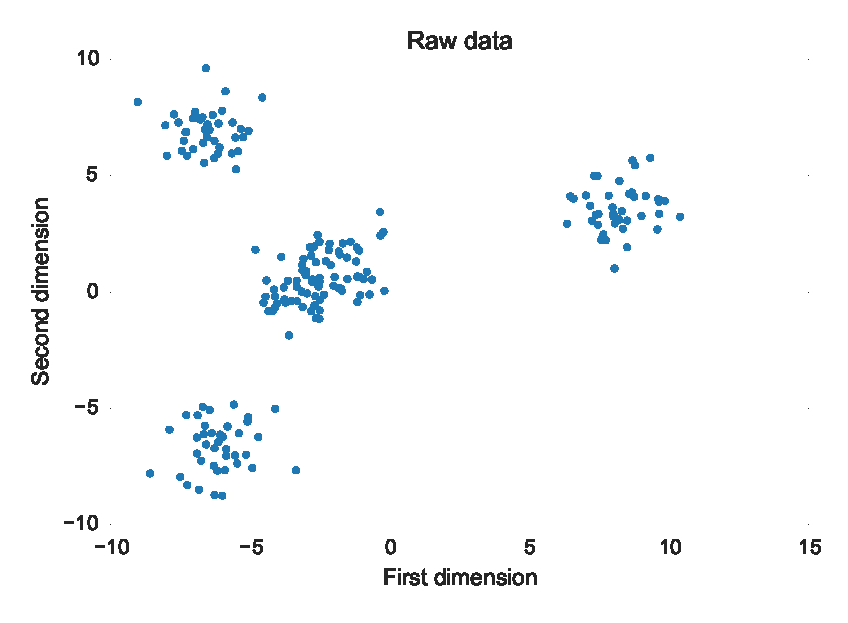
\includegraphics[scale=0.5]{introduction/img/cluster_example_raw.eps}
% \caption{Gaussian mixture of 5 distributions. The middle "ball" of points is 2 Gaussians that intersect.}
% \label{fig:intro raw}
% \end{figure}

% \begin{figure}[hbtp]
% \centering
% 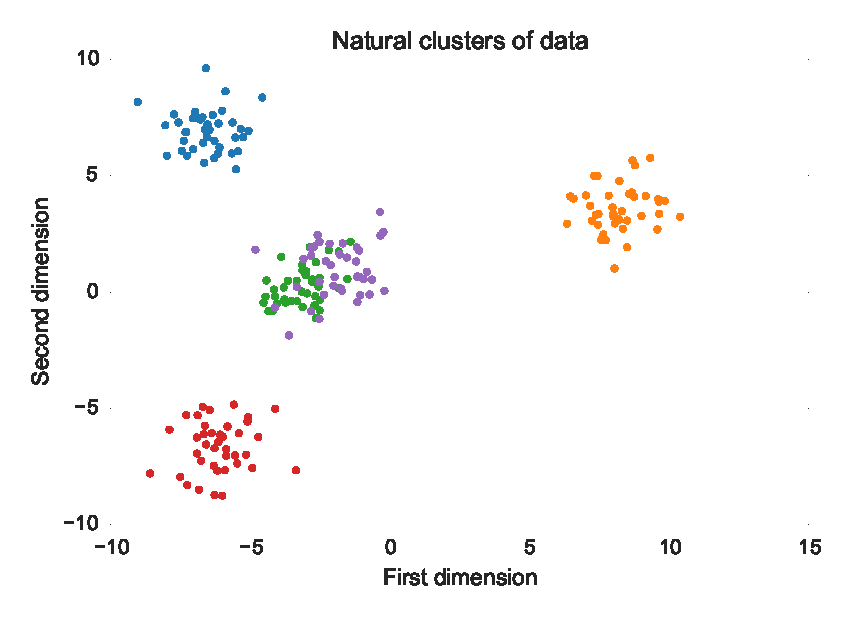
\includegraphics[scale=0.5]{introduction/img/cluster_example_natural.eps}
% \caption{Gaussian mixture of 5 distributions. The colors of each point represents the group (the Gaussian distribution) to which it belongs.}
% \label{fig:intro natural}
% \end{figure}

% \begin{figure}[hbtp]
% \centering
% 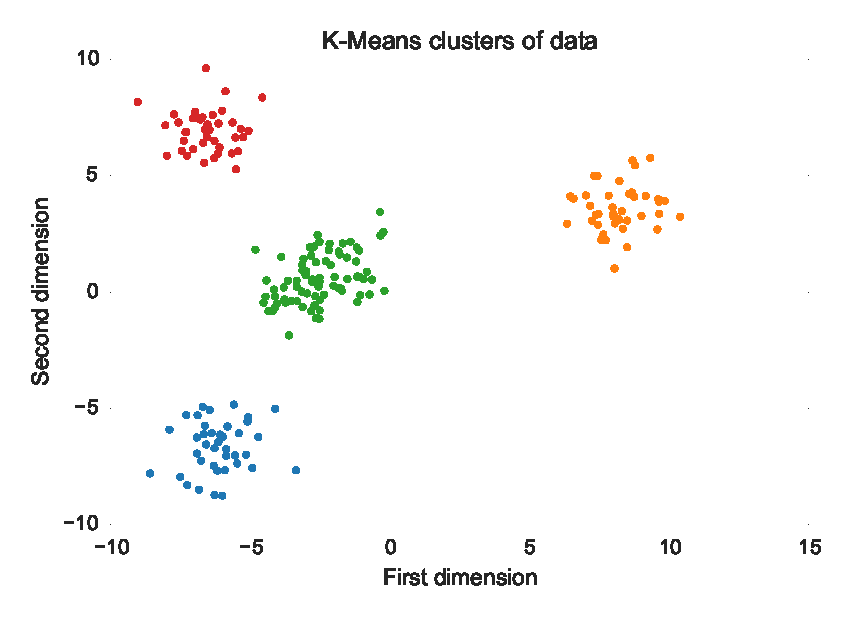
\includegraphics[scale=0.5]{introduction/img/cluster_example_kmeans.eps}
% \caption{Sama data, as Figure \ref{fig:intro raw}, but the group to which each point belongs to was computed by the K-Means algorithm with the number of clusters set to 4.}
% \label{fig:intro kmeans}
% \end{figure}

\begin{figure}[!ht]
    \centering
    \begin{subfigure}[b]{0.3\textwidth}
        \centering
        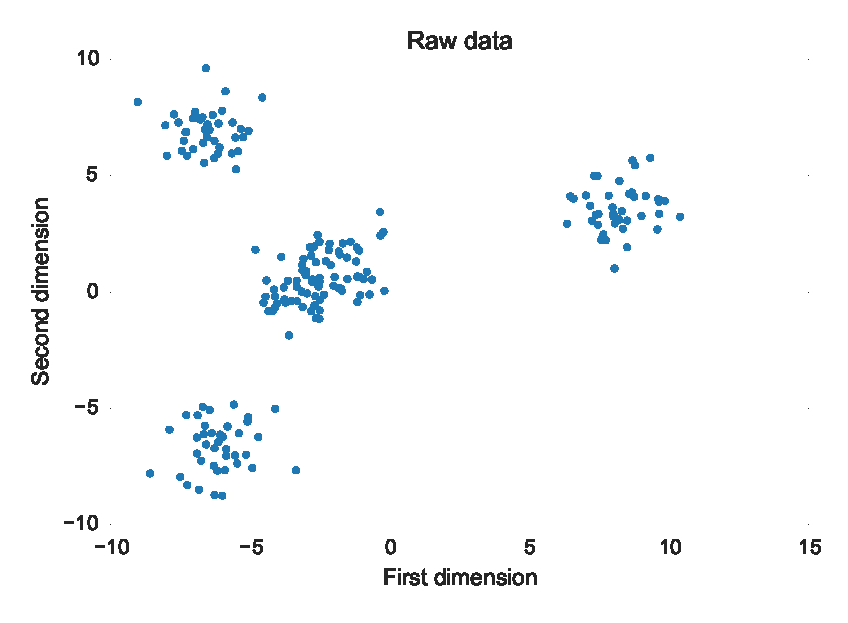
\includegraphics[width=\textwidth]{introduction/img/cluster_example_raw}
        \caption{Input data, unlabeled.}
        \label{fig:intro raw}
    \end{subfigure}
    \hfill
    \begin{subfigure}[b]{0.3\textwidth}
        \centering
        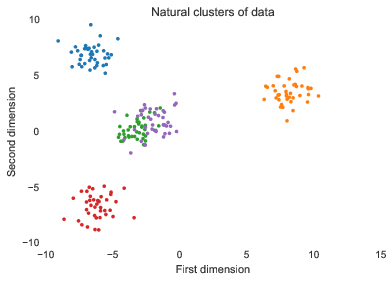
\includegraphics[width=\textwidth]{introduction/img/cluster_example_natural}
        \caption{Desired labels.}
        \label{fig:intro natural}
    \end{subfigure}
    \hfill
    \begin{subfigure}[b]{0.3\textwidth}
        \centering
        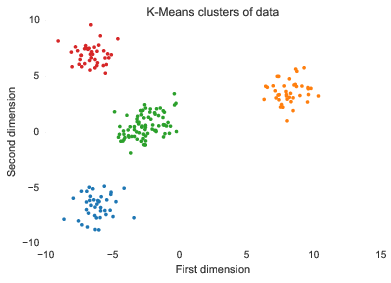
\includegraphics[width=\textwidth]{introduction/img/cluster_example_kmeans}
        \caption{K-Means's labels.}
        \label{fig:intro kmeans}
    \end{subfigure}
    \caption{Gaussian mixture of 5 distributions. Fig. \ref{fig:intro raw} shows the raw input data, i.e. how the algorithms "sees" the data. Fig. \ref{fig:intro natural} shows the desired labels for each point, which here means their corresponding Gaussian. Fig. \ref{fig:intro kmeans} shows the output labels of the K-Means algorithm with the number of clusters (input parameter) set to 4.}
    \label{fig:clustering plots}
\end{figure}


Cluster analysis is a relevant technique across several domains (\cite{Aggarwal2014}):

\begin{itemize}
	\item grouping users with similar behaviour or preferences in \textbf{customer segmentation};
	\item image segmentation in the field of \textbf{image processing};
	\item clustering gene expression data, among other application, in the domain of \textbf{biological data analysis};
	\item generation of hierarchical structure for easy access and retrieval of \textbf{information systems}; % not referenced in book
\end{itemize}

% Clustering is used in a wide variety of fields to solve numerous problems, e.g.:
% %TODO provide references to all of this
% % see https://sites.google.com/site/dataclusteringalgorithms/clustering-algorithm-applications
% % has applications with articles
% \begin{itemize}
% \item image segmentation in the field of image processing;
% \item generation of hierarchical structure for easy access and retrieval of information systems;
% \item recommender systems by grouping users by their behaviour and/or preferences;
% \item clustering customers for targeted marketing in 
% \item clustering gene expression data in biology;
% \item grouping of 
% \end{itemize} % file "Thesis_Introduction.tex"
\section{State of the art}

%TODO
% see if this is an apropriate structure; a quantum clustering section makes sense at the very least, but it should be introduced before

\subsection{Big data clustering}

\subsection{Quantum clustering}
The field of quantum computing has shown promising results regarding potential speedups in several tasks over their classical counterparts. 
There are two major paths for the problem of quantum clustering. The first is the quantization of clustering methods to work in quantum computers. This translates in converting algorithms to work partially or totally on a different computing paradigm, with support of quantum circuits or quantum computers. Literature suggests that quadratic (and even exponential in some cases) speedup may be achieved. Most of the approaches for such conversions make use of Groover's search algorithm, or a variant of it, e.g. [1]. Most literature on this path is also mostly theoretical since quantum circuits are not easily available and a working feasible quantum computer has yet to be invented. This path can be seen as part of the bigger problem of quantum computing and quantum information processing.

% #TODO get refs for simulation of quantum systems not being feasable; Feynmann; I think washington course had something -->

An alternative to using real quantum systems would be to simulate them. However, simulating quantum systems is a very hard task by itself and literature suggest is not feasible. Given that the scope of the thesis is to accelerate clustering, having the extra overhead of simulating the systems would allow speedups.

The second path is the computational intelligence approach, i.e.  to use quantum inspired algorithms that muster inspiration from quantum analogies. A study of the literature will reveal that this path typically further divides itself into two other branches. One comprehends the algorithms based on the concept of the quantum bit, the quantum analogue of a classical bit with interesting properties found in quantum objects. The other branch models data as a quantum system and uses the Schrödinger equation to evolve it.

In the following two sections these approaches for quantum inspired computational intelligence are explored.

[1] N. Wiebe, A. Kapoor, and K. Svore, “Quantum Algorithms for Nearest-Neighbor Methods for Supervised and Unsupervised Learning,” p. 31, 2014.

\subsubsection{Quantum bit}

The quantum bit is a quantum object that has the properties of quantum superposition, entanglement and ...

% taken from notebook -->

A qubit can have any value between 0 and 1 (superposition property) until it is observed, which is when the system collapses to either state. However, the probability with which the system collapses to either state  may be different. The superposition property or linear combination of states can be expressed as

$$
[\psi] = \alpha[0] + \beta[1]
$$

where $\psi$ is an arbitrary state vector and $\alpha$, $\beta$ are the the probability amplitude coefficients of basis states $[0]$ and $[1]$, respectevely. The basis states correspond to the spin of the modeled particle (in this case, a ferminion, e.g. electron). The coefficients are subjected to the following normalization:

$$|\alpha|^2 + |\beta|^2 = 1$$

where $|\alpha|^2$, $|\beta|^2$ are the probabilities of observing states $[0]$ and $[1]$, respectevely. $\alpha$ and $\beta$ are complex quantities and represent a qubit:

$$\begin{bmatrix}
\alpha \\
\beta
\end{bmatrix}$$

Moreover, a qubit string may be represented by:
$$
\begin{bmatrix}
\left.\begin{matrix}
\alpha_1\\ 
\beta_1
\end{matrix}\right| & \left.\begin{matrix}
\alpha_2\\ 
\beta_2
\end{matrix}\right| & \begin{matrix}
\alpha_3\\ 
\beta_3
\end{matrix}
\end{bmatrix}
$$

The probability of observing the state $[000]$ will be $|\alpha_1|^2 \times |\alpha_2|^2 \times |\alpha_3|^2$

To use this model for computing purposes, black-box objects called *oracles* are used.

% end of notebook -->

% #TODO get ref -->
Def from wiki: In complexity theory and computability theory, an oracle machine is an abstract machine used to study decision problems. It can be visualized as a Turing machine with a black box, called an oracle, which is able to decide certain decision problems in a single operation. The problem can be of any complexity class. Even undecidable problems, like the halting problem, can be used. %from http://en.wikipedia.org/wiki/Oracle_machine

In this context, oracles contain strings of qubits and generate their own input by observing the state of the qubits. After collapsing, the qubit value becomes analogue to a classical bit.

% #TODO get ref : see washington quantum computing classes -->
As it stands, oracles aren't quantum systems or even simulate them. The most appropriate description would be a probabilistic Turing machine.

Each string of qubits represents a number, so the number of qubits in each string will define its precision. The number of strings chosen for the oracles depends on the number of clusters and dimensionality of the problem (e.g. for 3 clusters of 2 dimensions, 6 strings will be used since 6 numbers are required). Each oracle will represent a possible solution.


\subsubsection{Quantum K-Means}

Several clustering algorithms [4-6], as well as optimization problems [7], are modelled after this concept. To test the potential of the algorithms under this paradigm, a quantum variant of the K-Means algorithm based on [5] was chosen as a case study.

\subsubsection{Description of the algorithm}

The Quantum K-Means (QK-Means) algorithm, as is described in [5], is based on the classical K-Means algorithm. It extends the basic K-Means with concepts from quantum mechanics (the qubit) and genetic algorithms.

% (describe algorithm... - from notebook) -->
The algorithm has the following steps:
\begin{enumerate}
\item Initialize population of oracles
\item Collapse oracles
\item K-Means
\item Compute cluster fitness
\item Store
\item Quantum Rotation Gate
\item Collapse oracles
\item Quantum cross-over and mutation
\item Repeat 3-7 until generation (iteration) limit is reached
\end{enumerate}



The algorithm implemented and tested is a variant of the one described in [5]. The genetic operations of cross-over and mutation are both part of the genetic algorithms toolbox, but were not implemented due to the suggestion from [1]. This decision was based on the findings of [8], stating that the use of the angle-distance rotation method in the quantum rotation operation produces enough variability, with a careful choice of the rotation angle.

\paragraph{Initialize population of oracles}

The oracles are created in this step and all qubit coefficients are initialized with $\frac{1}{\sqrt{2}}$, so that the system will observe either state with equal probability. This value is chosen taken into account the necessary normalization of the coefficients.

\paragraph{Collapse oracles}

Collapsing the oracles implies making an observation of each qubit of each qubit string in each oracle. This is done by first choosing a coefficient to use (either can be used), e.g. $\alpha$. Then, a random value $r$ between 0 and 1 is generated. If $\alpha \ge r$ then the system collapses to $[0]$, otherwise to $[1]$.

\paragraph{K-Means}
In this step we convert the binary representation of the qubit strings to base 10 and use them those values as initial centroids for K-Means. For each oracle, classical K-Means is then executed until it stabilizes or reaches the iteration limit. The solution centroids are returned to the oracles in binary representation.

\paragraph{Compute cluster fitness}
Cluster fitness is computed using the Davies-Bouldin index for each oracle. The score of each oracle is stored in the oracle itself.

\paragraph{Store}
The best scoring oracle is stored.

\paragraph{Quantum Rotation Gate}
So far, we've had classical K-Means with a complex random number generation for the centroids and complicated data structures. This is the step that fundamentally differs from the classical version. In this step a quantum gate (in this case a rotation gate) is applied to all oracles except the best one. The basic idea is to shift the qubit coefficients of the least scoring oracles so they'll have a higher probability of collapsing into initial centroid values closer to the best solution so far. This way, in future generations, we'll not initiate with the best centroids so far (which will not converge further into a better solution) but we'll be closer while still ensuring diversity (which is also a desired property of the genetic computing paradigm). In conclusion, we want to look for better solutions than the one we got before in each oracle while moving in the direction of the best we found so far.

% (end of notebook entry) -->

The other approach to clustering that gathers inspiration from quantum mechanical concepts is to use the Schrödinger equation. The algorithm under study was created by Horn and Gottlieb and was later extended by Weisenberg? and Horn.

%TODO
% add ref

\subsubsection{Horn and Gottlieb's algorithm}

The first step in this methodology is to compute a probability density function of the input data. This is done with a Parzen-window estimator in [2,3]. This function will be the wave function in the Schrödinger equation. Having this information we'll compute the potential function that corresponds to the state of minimum energy (ground state = eigenstate with minimum eigenvalue) [2].

This potential function is akin to the inverse of a probability density function. Minima of the potential correspond to intervals in space where points are together. So minima will naturally correspond to cluster centres [2]. The potential of every point in space is a costly computation. One method to address this problem is to compute the potential on the input data and converge this points toward some minima of the potential function. This is done with the gradient descent method in [2]. Another method [3] is to think of the input data as particles and use the Hamiltonian operator to evolve the quantum system in the time-dependant Schrödinger equation. Given enough time steps, the particles will converge to and oscillate around potential minima.

Both methods take as input parameter the variance $\sigma$ of the parzen-window estimator.

% (from notebook Horn accuracy) -->
This method starts off by creating a Parzen-window density estimation of the input data by associating a Gaussian with each point, such that

$$ \psi (\mathbf{x}) = \sum ^N _{i=1} e^{- \frac{\left \| \mathbf{x}-\mathbf{x}_i \right \| ^2}{2 \sigma ^2}} $$

where $N$ is the total number of points in the dataset, $\sigma$ is the variance and $\psi$ is the probability density estimation. $\psi$ is chosen to be the wave function in Schrödinger's equation. The details of why this is are better described in [1-4]. Schrödinger's equation is solved in order of the potential function $V(x)$, whose minima will be the centres of the clusters of our data:      

$$
V(\mathbf{x}) = E + \frac {\frac{\sigma^2}{2}\nabla^2 \psi }{\psi} 
= E - \frac{d}{2} + \frac {1}{2 \sigma^2 \psi} \sum ^N _{i=1} \left \| \mathbf{x}-\mathbf{x}_i \right \| ^2 e^{- \frac{\left \| \mathbf{x}-\mathbf{x}_i \right \| ^2}{2 \sigma ^2}}
$$

And since the energy should be chosen such that $\psi$ is the groundstate (i.e. eigenstate corresponding to minimum eigenvalue) of the Hamiltonian operator associated with Schrödinger's equation (not represented above), the following is true

$$
E = - min \frac {\frac{\sigma^2}{2}\nabla^2 \psi }{\psi}
$$

With all of this, $V(x)$ can be computed. However, it's very computationally intensive to compute V(x) to the whole space, so we only compute the value of this function close to the data points. This should not be problematic since clusters' centres are generally close to the data points themselves. Even so, the minima may not lie on the data points themselves, so what we do is compute the potential at all data points and then apply the gradient descent method to move them to regions in space with lower potential.

There is another method to evolve the system other then by gradient descent which is explained in [4]. Together, this methods make the Dynamic Quantum Clustering algorithm % #TODO add ref -->.
% (continue) -->

% #TODO describe the fine cluster algorithm; critique how this is done; what was developed; what  -->


%[1] N. Wiebe, A. Kapoor, and K. Svore, “Quantum Algorithms for Nearest-Neighbor Methods for Supervised and Unsupervised Learning,” p. 31, 2014.
%
%[2] D. Horn and A. Gottlieb, “The Method of Quantum Clustering.,” NIPS, no. 1, 2001.
%[3] M. Weinstein and D. Horn, “Dynamic quantum clustering: a method for visual exploration of structures in data,” Phys. Rev. E - Stat. Nonlinear, Soft Matter Phys., vol. 80, no. 6, pp. 1–15, Dec. 2009.
%
%[4] E. Casper and C. Hung, “Quantum Modeled Clustering Algorithms for Image Segmentation,” vol. 2, no. March, pp. 1–21, 2013.
%[5] E. Casper, C.-C. Hung, E. Jung, and M. Yang, “A Quantum-Modeled K-Means Clustering Algorithm for Multi-band Image Segmentation.” [Online]. Available: http://delivery.acm.org/10.1145/2410000/2401639/p158-casper.pdf?ip=193.136.132.10&id=2401639&acc=ACTIVE SERVICE&key=2E5699D25B4FE09E.F7A57B2C5B227641.4D4702B0C3E38B35.4D4702B0C3E38B35&CFID=476955365&CFTOKEN=55494231&__acm__=1423057410_0d77d9b5028cb3. [Accessed: 04-Feb-2015].
%[6] J. Xiao, Y. Yan, J. Zhang, and Y. Tang, “A quantum-inspired genetic algorithm for k-means clustering,” Expert Syst. Appl., vol. 37, pp. 4966–4973, 2010.
%
%[7] H. Wang, J. Liu, J. Zhi, and C. Fu, “The Improvement of Quantum Genetic Algorithm and Its Application on Function Optimization,” vol. 2013, no. 1, 2013.
%
%[8] W. Liu, H. Chen, Q. Yan, Z. Liu, J. Xu, and Y. Zheng, “A novel quantum-inspired evolutionary algorithm based on variable angle-distance rotation,” 2010 IEEE World Congr. Comput. Intell. WCCI 2010 - 2010 IEEE Congr. Evol. Comput. CEC 2010, 2010.


\subsection{Parallel computing}
The second direction of the work was given to parallel computing, more spefically to General-Purpose Computation on Graphics Processing Units (GPGPU). 

\subsubsection{Short Survey of available GPGPU frameworks}


\subsubsection{Comparison and choice}
It basically boils down to OpenCL vs CUDA. OpenCL has the advantage of portability with the issues of performance portability and hard to program. Programming under CUDA, performs well since it was designed alongside with the hardware itself but only works on NVIDIA devices.

\subsubsection{Overview of CUDA}

 % add new .tex files for new chapters
%!TEX root = thesis.tex

\chapter{Methodology}
\label{chapter:methodology}


%TODO explain methodology to obtain results of quantum clustering of just present results on why it wasn't viable?

%TODO This is where I explain my approach to the problem of EAC in Big Data

The aim of this thesis is the optimization and scalability of EAC, with a focus for big data. EAC is divided in three steps and each has to be considered for optimization.

The first step is the accumulation of evidence, i.e. generating an ensemble of partitions. The main objective for the optimization of this step is speed. Using fast clustering methods for generating partitions is an obvious solution, as is the optimization of particular algorithms aiming for the same objective. Since each partition is independent from every other partition, parallel computing over a cluster of computing units would result in a fast ensemble generation. Using either or any combination of these strategies will guarantee a speedup. Furthermore, it is not necessary for algorithms to produce accurate clusterings, e.g. K-Means doesn't have to converge - 3 iterations should suffice. The reason for this is the want for variability within the partition population.
	
The second step is mostly bound by memory. The complete co-association matrix has a space complexity of $\mathcal{O}(n^2)$. Such complexity becomes prohibitive for big data, e.g. a dataset of $2 \times 10^6$ samples will result in a complete co-association matrix of $14901 \; GB$ if values are stored in single floating-point precision.

The last step has to take into account both memory and speed requirements. The final clustering must be able to produce good results, fast while not exploding the already big space complexity from the co-association matrix.

Initial research was under the field of quantum clustering. After this pursuit proved fruitless regarding one of the main requirements (computational speed), the focus of researched shifted to parallel computing, more specifically GPGPU. 

\section{Quantum Clustering}

Research under this paradigm aimed to find a solution for the first and last steps. Two venues were explored: Quantum K-Means and Horn and Gottlieb's quantum clustering algorithm.
For both, the experiments that were setup had the goal of evaluating the speed and accuracy performances of the algorithms.

Under the qubit concept, no other algorithms were experimented with since the results for this particular algorithm showed that this kind of approach is infeasible due to the cost in computational speed. The results highlight that fact.



\section{Speeding up Ensemble Generations with Parallel K-Means}
K-Means is an obvious candidate for the generation of partitions since it is simple, fast and partitions don't require big accuracy - variability in the partitions is a desirable property which translates in few iterations. For that reason, optimizing this algorithm would ensure that the accumulation of evidence would be performed in an efficient manner.



%TODO pseudocode & diagrams
%TODO explain the solution for GPGPU K-Means

\section{Dealing with space complexity of coassocs}
In the literature review, two approaches to deal with the space complexity of the co-association matrix were reported. It would be ideal to combine both approaches to further reduce space complexity, but they're not compatible as it might seem. When the neighbour approach is used, it is unlikely that a sample will never be clustered with it's closest $p$ neighbours. This means that the $n \times p$ co-association matrix will likely not have many zeros which translates in little return for using the sparsity augmentation approach. To illustrate this point, let's consider a dataset of $10^6$ patterns. 

%comment on which method is more effective, maybe some experiment is needed to see which
%demonstrate why both methods are not compatible - a simple filling of knn matrix should suffice

Which method is more effective in very large datasets, however, would depend on the dataset. The sparsity maximization approach got very low densities for some datasets, close to $0.01$ in some cases. This is already a very improvement

Either way, the CSR data structure is used to store the co-association matrix. 
Due to the sparse nature of the co-association matrix this can decrease used space to as much as $10\%$, depending on the sparsity of the matrix as shown in \cite{Lourenco2010}. 
This is important since in this way the co-association matrix is already in the correct format for the next step - the computation of the MST for the HAC.

\section{Accelerating HAC}

The final clustering, done with SL-HAC, is optimized by executing the efficient parallel variant of Borůvka's algorithm \cite{Sousa2015} with a slight modification for accepting unconnected graphs, i.e. a co-association matrix where there may be a pattern or a group of patterns that are not connected to any other pattern.
In the present implementation, the issue of unconnected graphs was solved in the first step of the efficient variant (finding the minimum vertex connected to each vertex or supervertex). If a vertex has no edges connected to it then it is marked as if its destination points to itself (as a mirrored edge in the second step). This results in unconnected vertices (or supervertices) being dragged throughout all the iterations.
As a consequence, the stopping criteria becomes the lack of edges connected to the remaining vertices, which is the same as saying that all elements of the \emph{outdegree} array are zero. This condition can be checked as a secondary result of the computation of the new \emph{first\_edge} array. This step is performed by applying an exclusive prefix sum over the \emph{outdegree}. If the prefix sum is implemented in such a way that it returns the sum of all elements, then it becomes inexpensive to check this condition.

The result of this variant is an array of length $|V|-1$, i.e. $N-1$ since the vertices are the patterns of the dataset. 



 % add new .tex files for new chapters
%!TEX root = thesis.tex


\section{Results}
\subsection{Quantum K-Means}


The algorithm implemented and tested is a variant of the one described in ~\cite{Casper}. The genetic operations of cross-over and mutation are both part of the genetic algorithms toolbox, but were not implemented due to the suggestion from ~\cite{Wiebe2014}. This decision was based on the findings of ~\cite{Liu2010}, stating that the use of the angle-distance rotation method in the quantum rotation operation produces enough variability, with a careful choice of the rotation angle.

\subsubsection{Testing and Results}
The testing was aimed at benchmarking both accuracy and speed. The input used was synthetic data, namely, Gaussian mixtures with variable cardinality and dimensionality. The algorithm was implemented in Python 2.7 and the tests were executed in a machine with an Intel i5 processor, 2GB RAM and running Ubuntu 14.04.

(copy of report)

Regarding the Quantum K-Means (QK-Means), the tests were performed using 10 oracles, a qubit string length of 8 and 100 generations per round. The \textbf{classical} K-Means was executed using the \textbf{k-means++} centroid initialization method, since QK-Means also has some computational cost in the beginning of the algorithm.. Since QK-Means executes a classical K-Means for each oracle each generation, the number of initializations for K-Means was $num.oracles \times num.generations \times factor$, where $factor$ is an adjustable multiplier. Each test had 20 rounds t allow for statistical analysis of the results.

All tests were done with 6 clusters (natural number of clusters). Two tests were done with the two dimensional dataset: one with a $factor=1.10$ (increase initializations by $10\%$) and another with $factor=1$. These tests will be called T1 and T2, respectively. The test done with the six dimensional dataset (T3) used $factor=1.10$.

Timing results

% table in csv format available in resource directory -->

\begin{table}[h]
\caption{Timing results for the different algorithms in the different tests. Fitness time refers to the time that took to compute the DB index of each solution of classical K-Means. All time values are the average over 20 rounds and are displayed in seconds.}
\begin{tabular}{|l|l|l|l|l|l|}
\hline
\textbf{Dataset}               & \textbf{Algorithm} & \textbf{Mean} & \textbf{Variance} & \textbf{Best} & \textbf{Worst} \\ \hline
\textbf{T1}                    & QK-Means           & 62.02642975   & 0.077065212       & 61.620424     & 62.579969      \\ \cline{2-6} 
\textbf{bi36}                  & K-Means            & 6.4774672     & 0.002501651       & 6.352554      & 6.585451       \\ \cline{2-6} 
\textbf{}                      & K-Means + fitness  & 70.2238286    & 0.022223755       & 69.889105     & 70.548572      \\ \cline{2-6} 
\textbf{}                      & fitness            & 63.7463614    & 0.019722105       & 63.536551     & 63.963121      \\ \hline
\textbf{T2}                    & QK-Means           & 64.22347165   & 0.056559152       & 63.807367     & 64.807373      \\ \cline{2-6} 
\textbf{bi36 noFactor} & K-Means            & 5.71167475    & 0.004903253       & 5.581391      & 5.877091       \\ \cline{2-6} 
\textbf{}                      & K-Means + fitness  & 62.7021533    & 0.066919692       & 63.417207     & 62.180021      \\ \cline{2-6} 
\textbf{}                      & fitness            & 56.99047855   & 0.062016439       & 56.59863      & 57.540116      \\ \hline
\textbf{T3}                    & QK-Means           & 74.4917966    & 0.067688312       & 74.12105      & 74.976446      \\ \cline{2-6} 
\textbf{sex36}                 & K-Means            & 8.291648      & 0.007015777       & 8.160859      & 8.426203       \\ \cline{2-6} 
                               & K-Means + fitness  & 72.36315915   & 0.05727269        & 71.856457     & 73.031841      \\ \cline{2-6} 
                               & fitness            & 64.07151115   & 0.050256913       & 63.695598     & 64.605638      \\ \hline
\end{tabular}
\end{table}

The mean computation time of classical K-Means is an order of magnitude lower than that of QK-Means. However, in classical K-Means the solution typically chosen is the one with lowest sum of squared euclidean distances of points to their attributed centroid. To make a fair comparison between the two algorithms, the Davies-Bouldin index of all classical K-Means solutions was computed and used as the criteria to choose the best solution. When this is done, we can see that the total time of classical K-Means is actually higher that that of QK-Means in T1 and T3, but this is only due to the 1.10 multiplier on the number of initializations. In T2, possibly the fairest comparison, the computation times become very similar with only a 2\% difference between the two algorithms.

Accuracy

Comparing K-Means and QK-Means

% table in csv format available in resource directory -->

\begin{table}[h]
\caption{All values displayed are the average over 20 rounds, except for the Overall best which shows the best result in any round. The values represent the Davies-Bouldin fitness index (low is better).}
\begin{tabular}{|l|l|l|l|l|l|l|}
\hline
\textbf{Dataset} & \textbf{Algorithm} & \textbf{Best} & \textbf{Worst} & \textbf{Mean} & \textbf{Variance} & \textbf{Overall best} \\ \hline
\textbf{T1}      & QK-Means           & 15.42531927   & 32.29577426    & 19.94704511   & 21.23544567       & 15.42531927           \\ \cline{2-7} 
\textbf{}        & K-Means            & 15.42531927   & 25.44913817    & 16.25013365   & 1.216919278       & 15.42531927           \\ \hline
\textbf{T3}      & QK-Means           & 22.72836641   & 65.19984617    & 36.10699242   & 78.14043743       & 22.71934191           \\ \cline{2-7} 
\textbf{}        & K-Means            & 22.71934191   & 46.72231967    & 26.18440481   & 22.96730826       & 22.71934191           \\ \hline
\end{tabular}
\end{table}

The most relevant result in the table above is the mean of the best index. The value is the average over all rounds of the best solution in each round and it provides insight on the average performance of the algorithm. The results suggest that both algorithms perform equally well. The best overall result of each algorithm in all rounds is exactly the same. In T3, the mean performance of classical K-Means is marginally better.

I speculate that if classical K-Means was using only the sum of euclidean distances and not the DB index, the average performance would be worse. As it stands, choosing to use DB index with classical K-Means possibly represents a tradeoff between speed and accuracy.

QK-Means details

Here we’ll analyse a bit what’s happening within each QK-Means execution. One would expect for the population’s fitness variance to decrease over the generations, as the probabilities for previous known solutions increase and are therefore more likely to reappear. The convergence of the population mean would also be expected to decrease for the same reason. However, experimental (Fig. \ref{fig:db_index_mean_t2} and \ref{fig:db_index_var_t2}) results don’t suggest any of these expectations (the results of T1 and T3 suggest the same). This may be due to low number of generations or simply because the random generation of initial centroids isn’t influenced enough by the qubit probabilities.


\begin{figure}[hbtp]
\centering
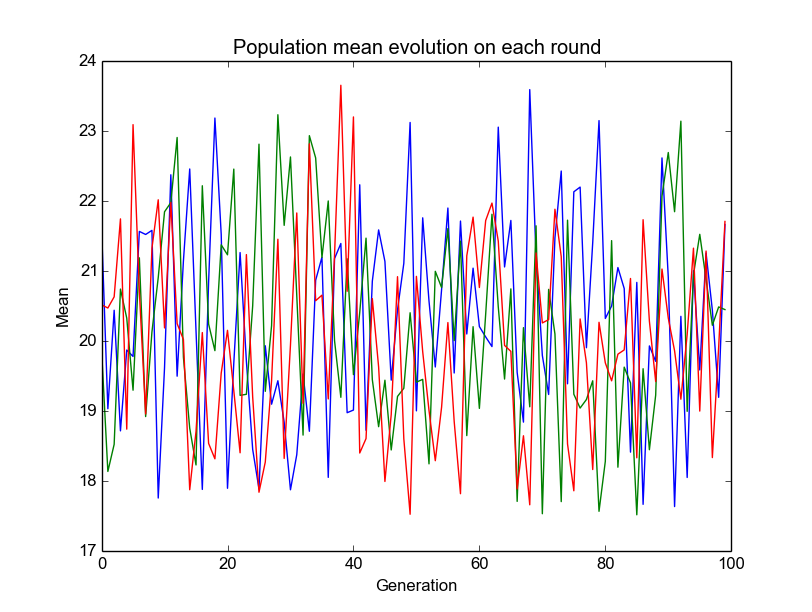
\includegraphics[scale=0.5]{QK_Means/img/bi_nofactor_mean.png}
\caption{DB index mean of the population in T2. Only 4 rounds represented.}
\label{fig:db_index_mean_t2}
\end{figure}

\begin{figure}[hbtp]
\centering
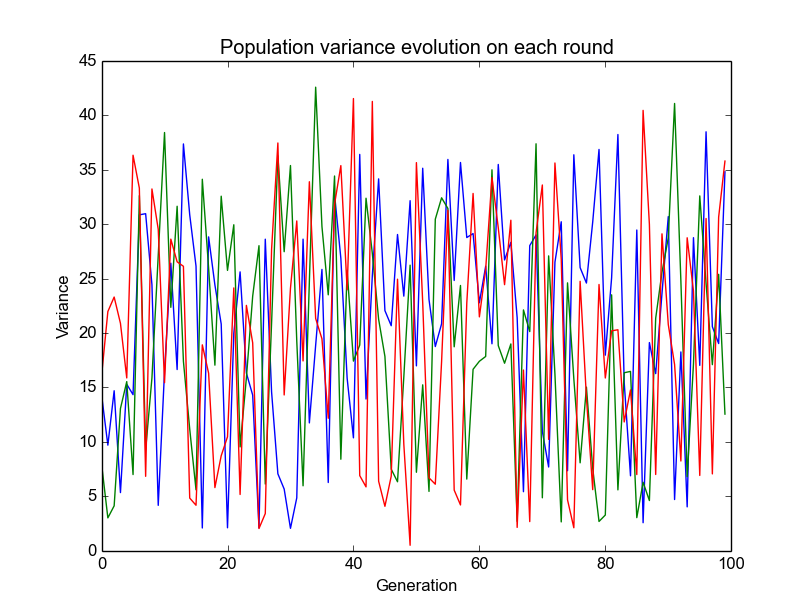
\includegraphics[scale=0.5]{QK_Means/img/bi_nofactor_var.png}
\caption{DB index variance of the population in T2. Only 4 rounds represented.}
\label{fig:db_index_var_t2}
\end{figure}


Analysing the evolution of the DB index of the best solution over the generations (Fig. \ref{fig:qk_db_index_best_evo_t2} and \ref{fig:qk_db_index_best_evo_t3}) gives some insight on the rate of convergence. In both tests it is clear that the best solution is often reached in a quarter of the total generations. More detail can be seen in the Table \ref{tab:db_index_t1_t3}.

\begin{figure}[hbtp]
\centering
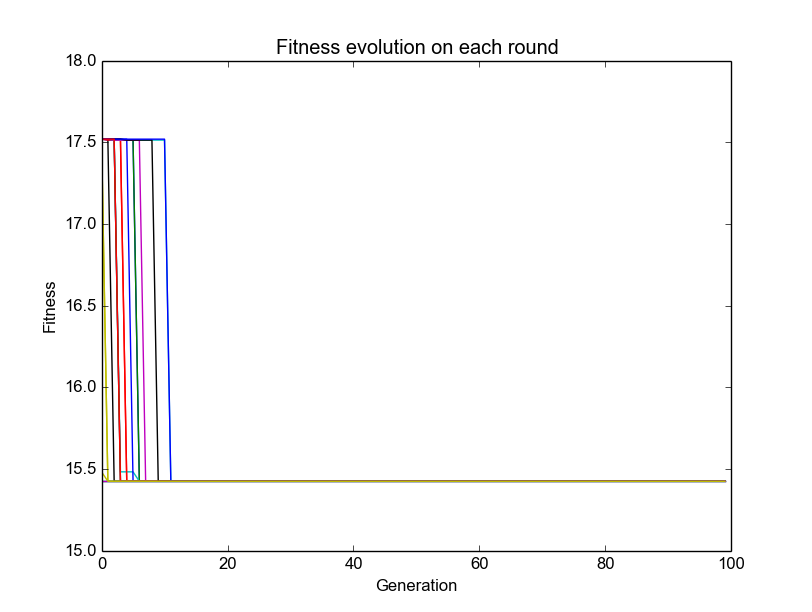
\includegraphics[scale=0.5]{QK_Means/img/bi_nofactor_evo.png}
\caption{DB index of best solution in T2.}
\label{fig:qk_db_index_best_evo_t2}
\end{figure}


\begin{figure}[hbtp]
\centering
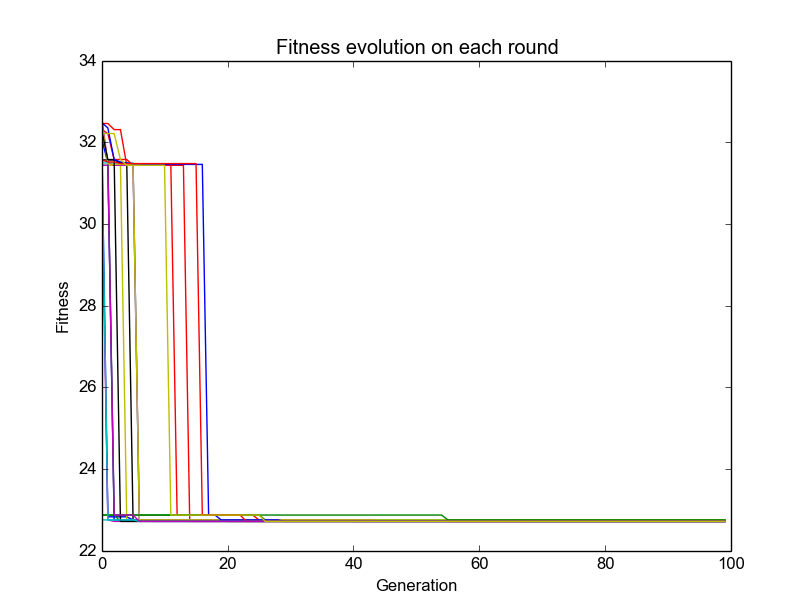
\includegraphics[scale=0.5]{QK_Means/img/sex_evo.png}
\caption{DB index of best solution in T3.}
\label{fig:qk_db_index_best_evo_t3}
\end{figure}

% table in csv format available in resource directory -->

\begin{table}[h]
\caption{The values represent generations.}
\begin{tabular}{|l|l|l|l|l|}
\hline
\textbf{Test} & \textbf{Mean} & \textbf{Variance} & \textbf{Best} & \textbf{Worst} \\ \hline
\textbf{T1}   & 17.25         & 70.2875           & 3             & 33             \\ \hline
\textbf{T3}   & 28.05         & 568.6475          & 2             & 90             \\ \hline
\end{tabular}
\label{tab:db_index_t1_t3}
\end{table}

\subsubsection{Discussion}

Results show that most computational cost (90\% on T1) lies on the evaluation of the solutions obtained from each oracle. This is a costly but necessary step in this algorithm. Moreover, and even though EAC doesn't require its input partitions to be accurate, the quality of the solutions, measured with the Davies-Bouldin index, from QK-Means doesn't differ from that of K-Means. This two facts make the use of this algorithm in EAC prohibitive, as no benefits in compuational time are gained.

It should be noted that the target application of the tests presented differs from that of the original authors and although no accuracy gains were observed in these results, the results might differ on different applications.

\subsection{Horn and Gottlieb's algorithm}


\subsubsection{Testing and Results}


%TODO
%Put in accuracy results for crab,iris and gaussian mixtures  
%Put in timing results


The accuracy of this algorithm was tested with real world datasets, namely, the crab and iris datasets available at the UCI Machine Learning Repository.

%TODO add ref for repository -->

\subsubsection{Iris data}
\label{sec:horn_iris}
The iris dataset ([available at the UCI ML repository](http://archive.ics.uci.edu/ml/datasets/Iris)) has 3 classes each with 50 data points. There are 4 features. The data is preprocessed using Principal Component Analysis (PCA). The natural clustering can be observed in Fig. \ref{fig:iris_natural}. 

% #TODO saved image from ipython -->

\begin{figure}[hbtp]
\centering
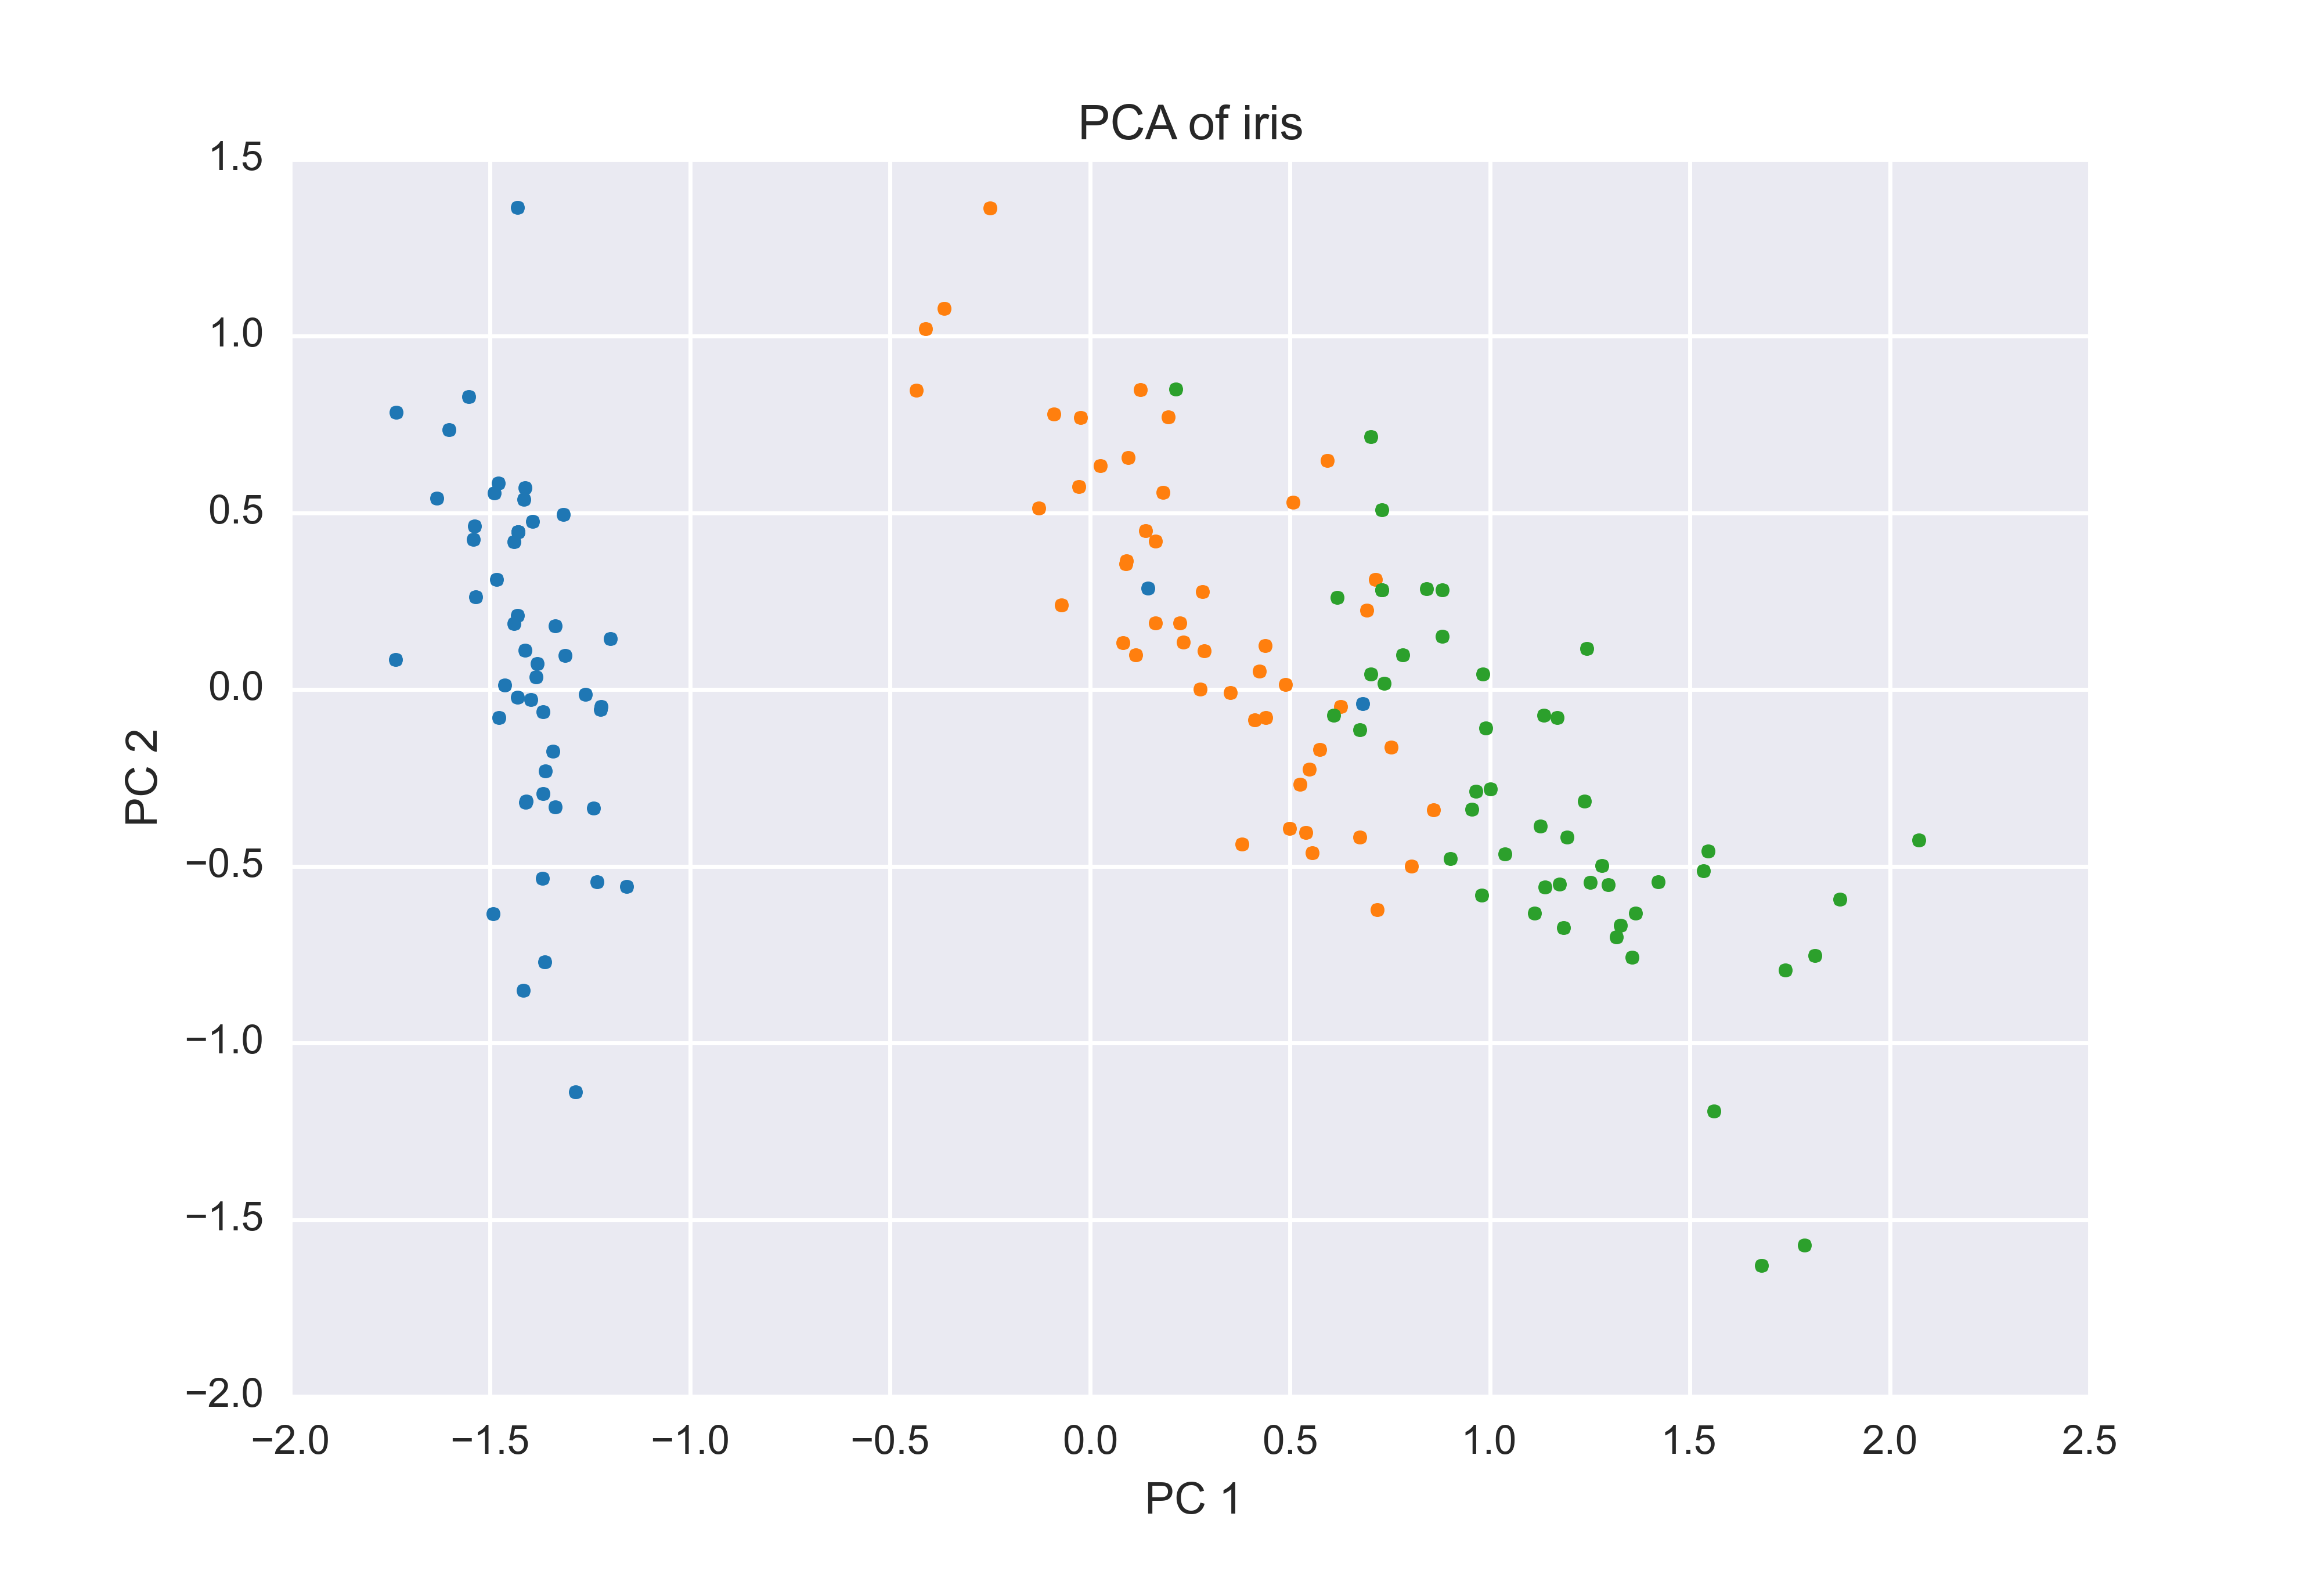
\includegraphics[scale=0.5]{Horn/img/iris_natural.png}
\caption{Plot of the two first principal components (PC).}
\label{fig:iris_natural}

\end{figure}

I chose $\sigma=\frac{1}{4}$ to reproduce the experiments in [3]. Only the first two PC are used here, which account for $95.8\%$ of the energy. The clustering results can be seen in Fig. \ref{fig:iris_2pc_cluster} and have an accuracy of 86\% computed with consistency index.


\begin{figure}[hbtp]
\centering
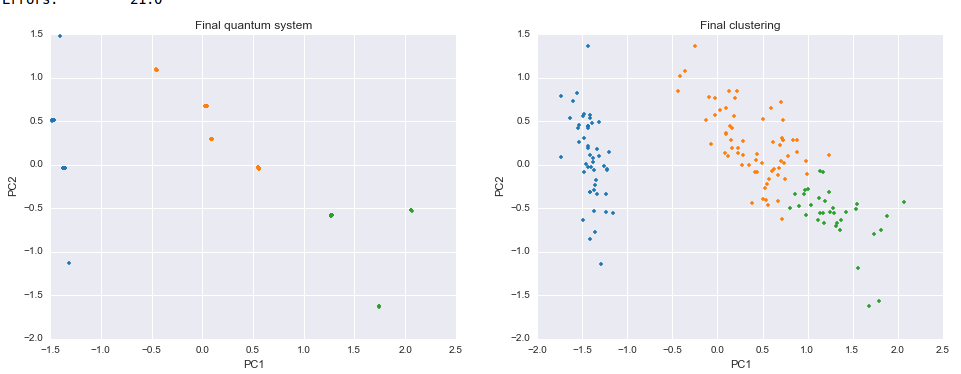
\includegraphics[width=\textwidth]{Horn/img/iris_2pc_cluster.png}
\caption{Plots of the converged data data points and final clustering for 2 PC.}
\label{fig:iris_2pc_cluster}

\end{figure}

For the sake of completeness, Fig. \ref{fig:iris_allpc_cluster} shows the clustering over all PCs. This solution has an accuracy of 82.67\% computed with consistency index.


\begin{figure}[hbtp]
\centering
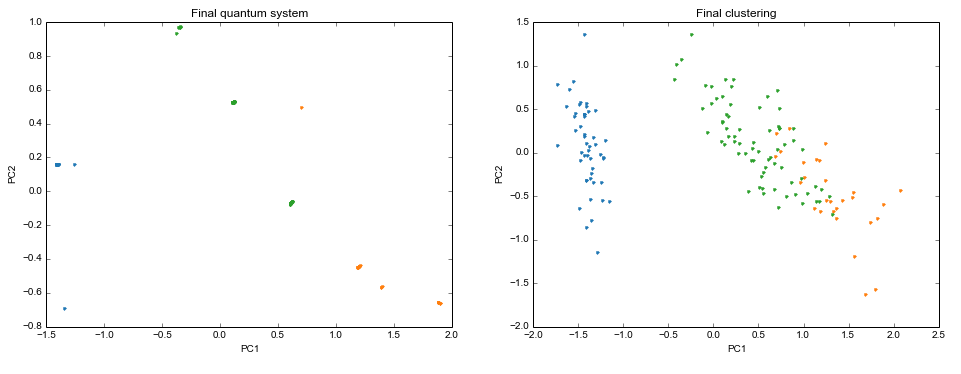
\includegraphics[width=\textwidth]{Horn/img/iris_allpc_cluster.png}
\caption{Plots of the converged data data points and final clustering for all PC of Iris data.}
\label{fig:iris_allpc_cluster}
\end{figure}


\subsubsection{Crab data}


The crabs dataset has 200 samples and describes 5 morphological measurements on 50 crabs each of two colour forms and both sexes (total of 200 crabs), of the species Leptograpsus variegatus collected at Fremantle, Western Australia. After a preprocessing using PCA with covariance matrix and uncentred data, the dataset is represented in Fig. \ref{fig:crab_2pc_covar}.% #TODO add reference to dataset -->

\begin{figure}[hbtp]
\centering
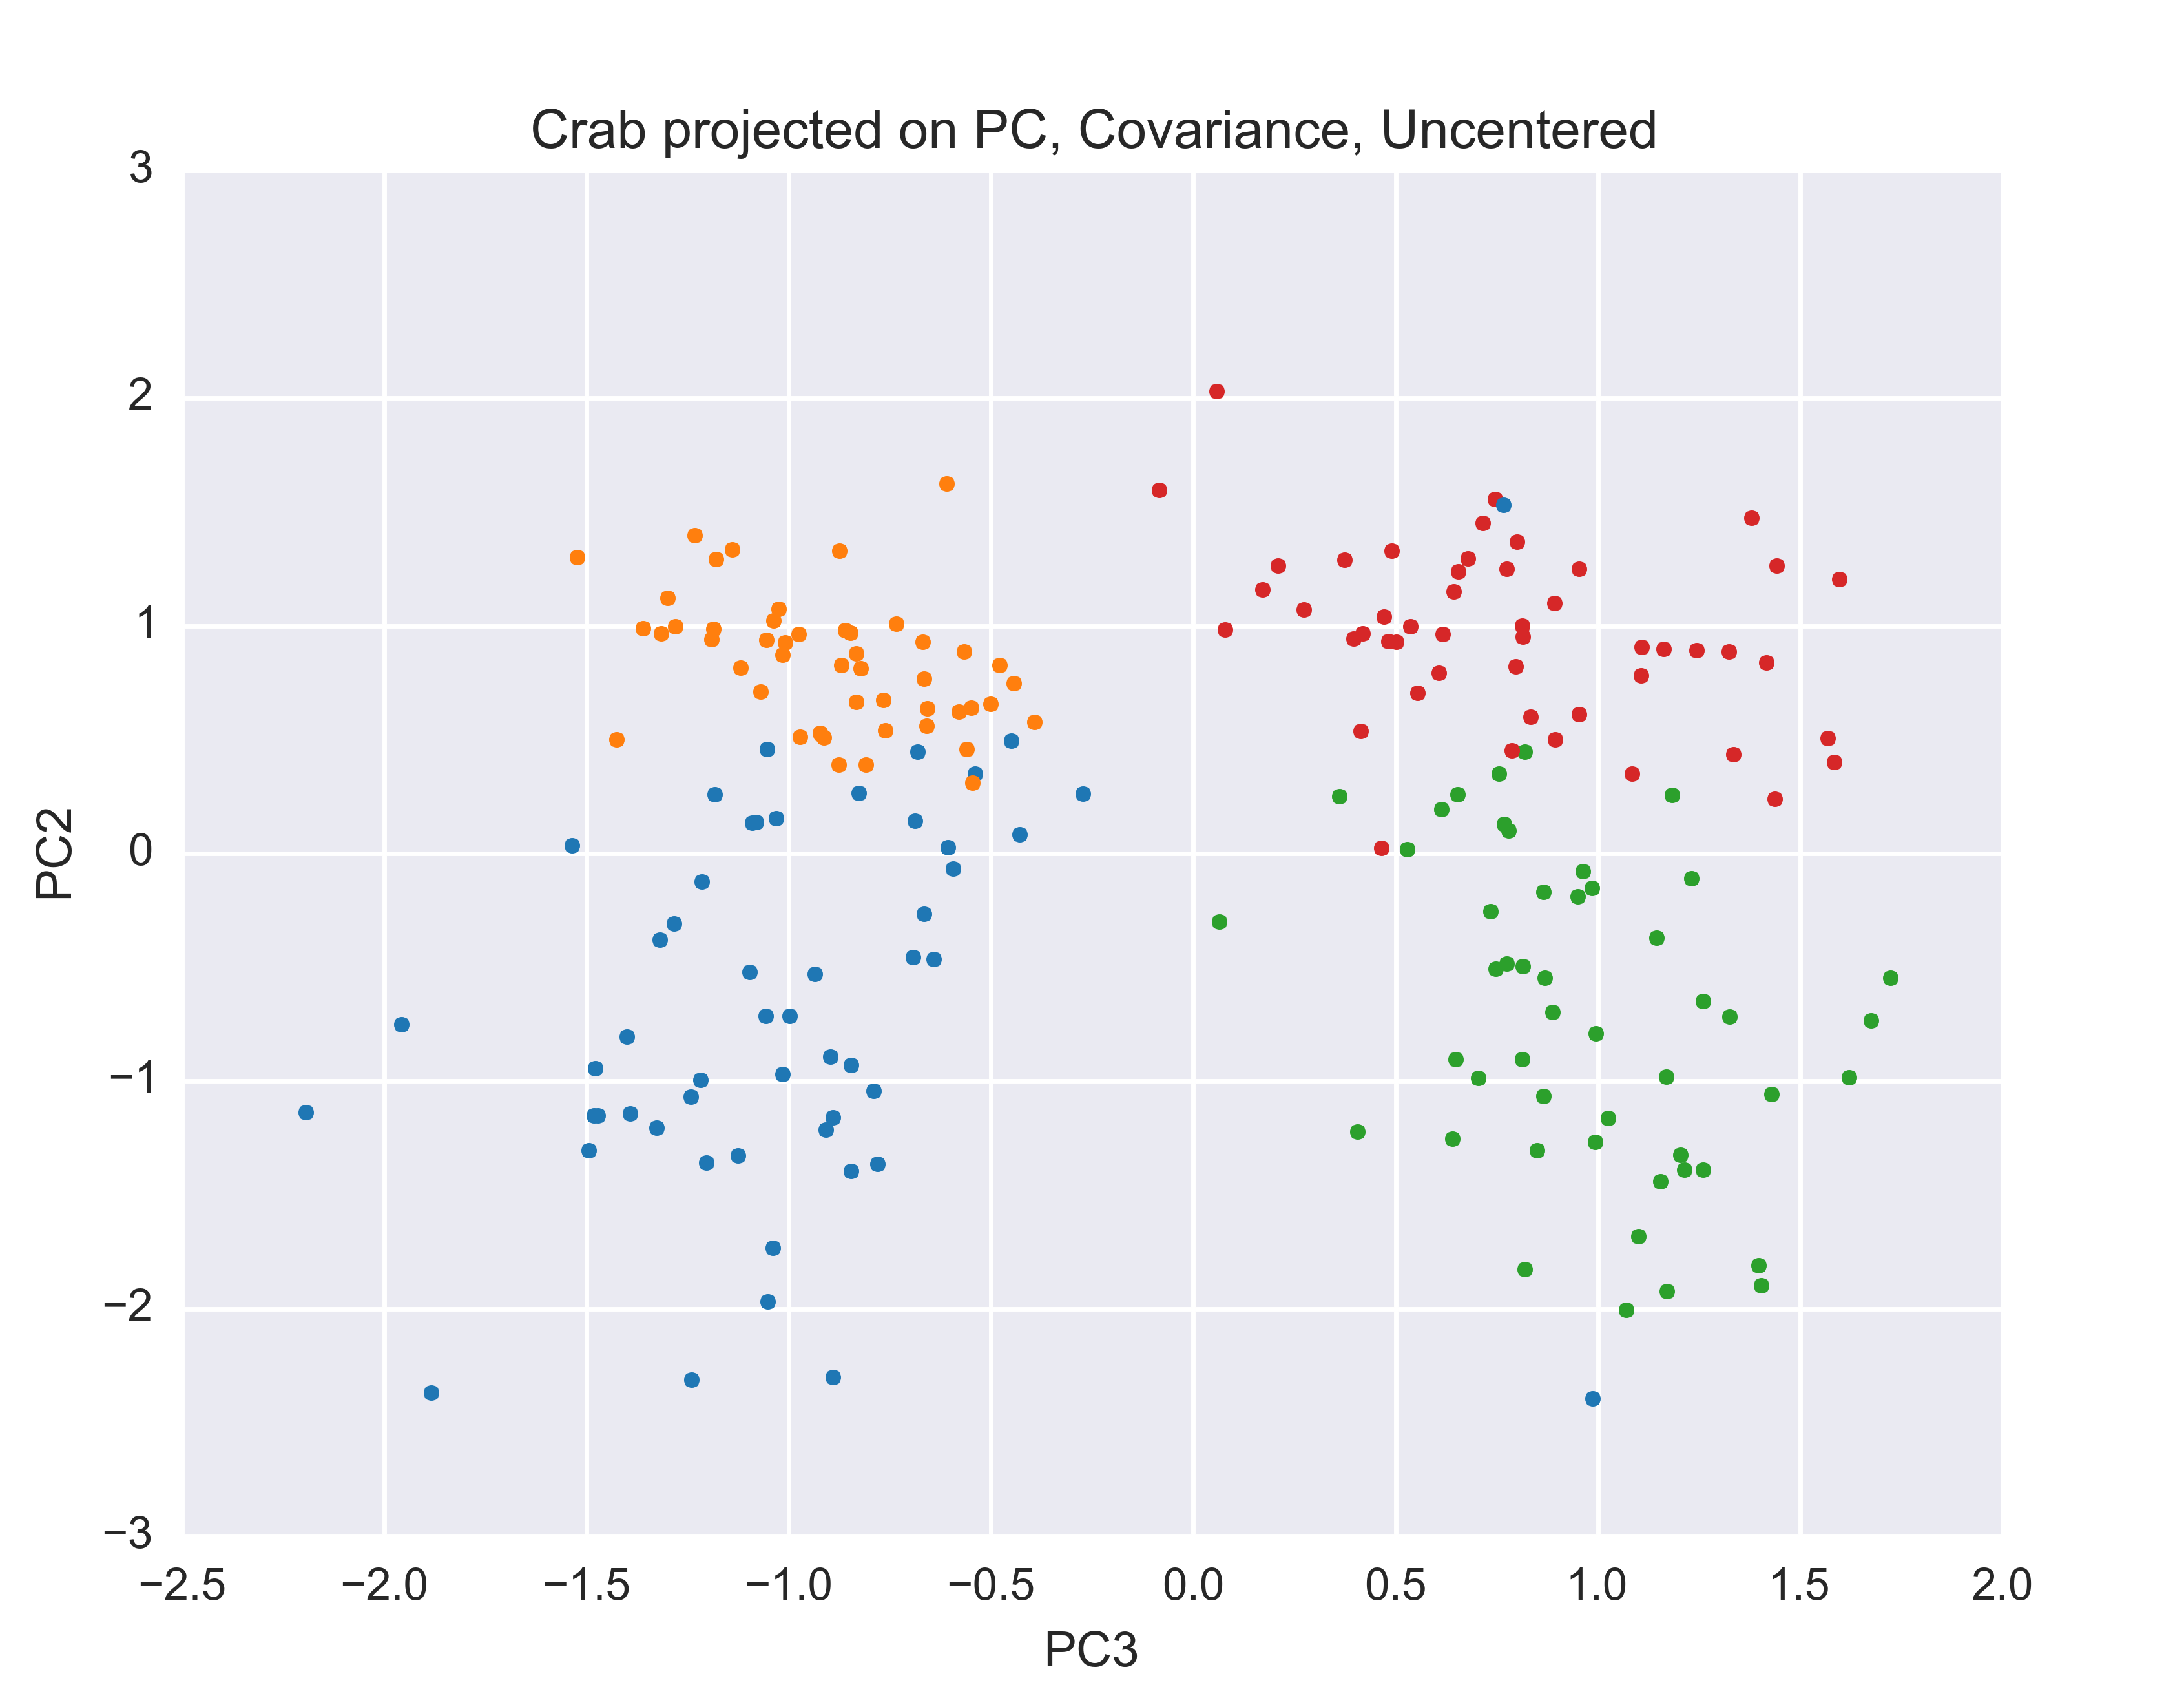
\includegraphics[scale=0.5]{Horn/img/crab_2pc_covar.png}
\caption{Representation of the crab data projected over PC 2 and 3.}
\label{fig:crab_2pc_covar}
\end{figure}

\begin{figure}[hbtp]
\centering
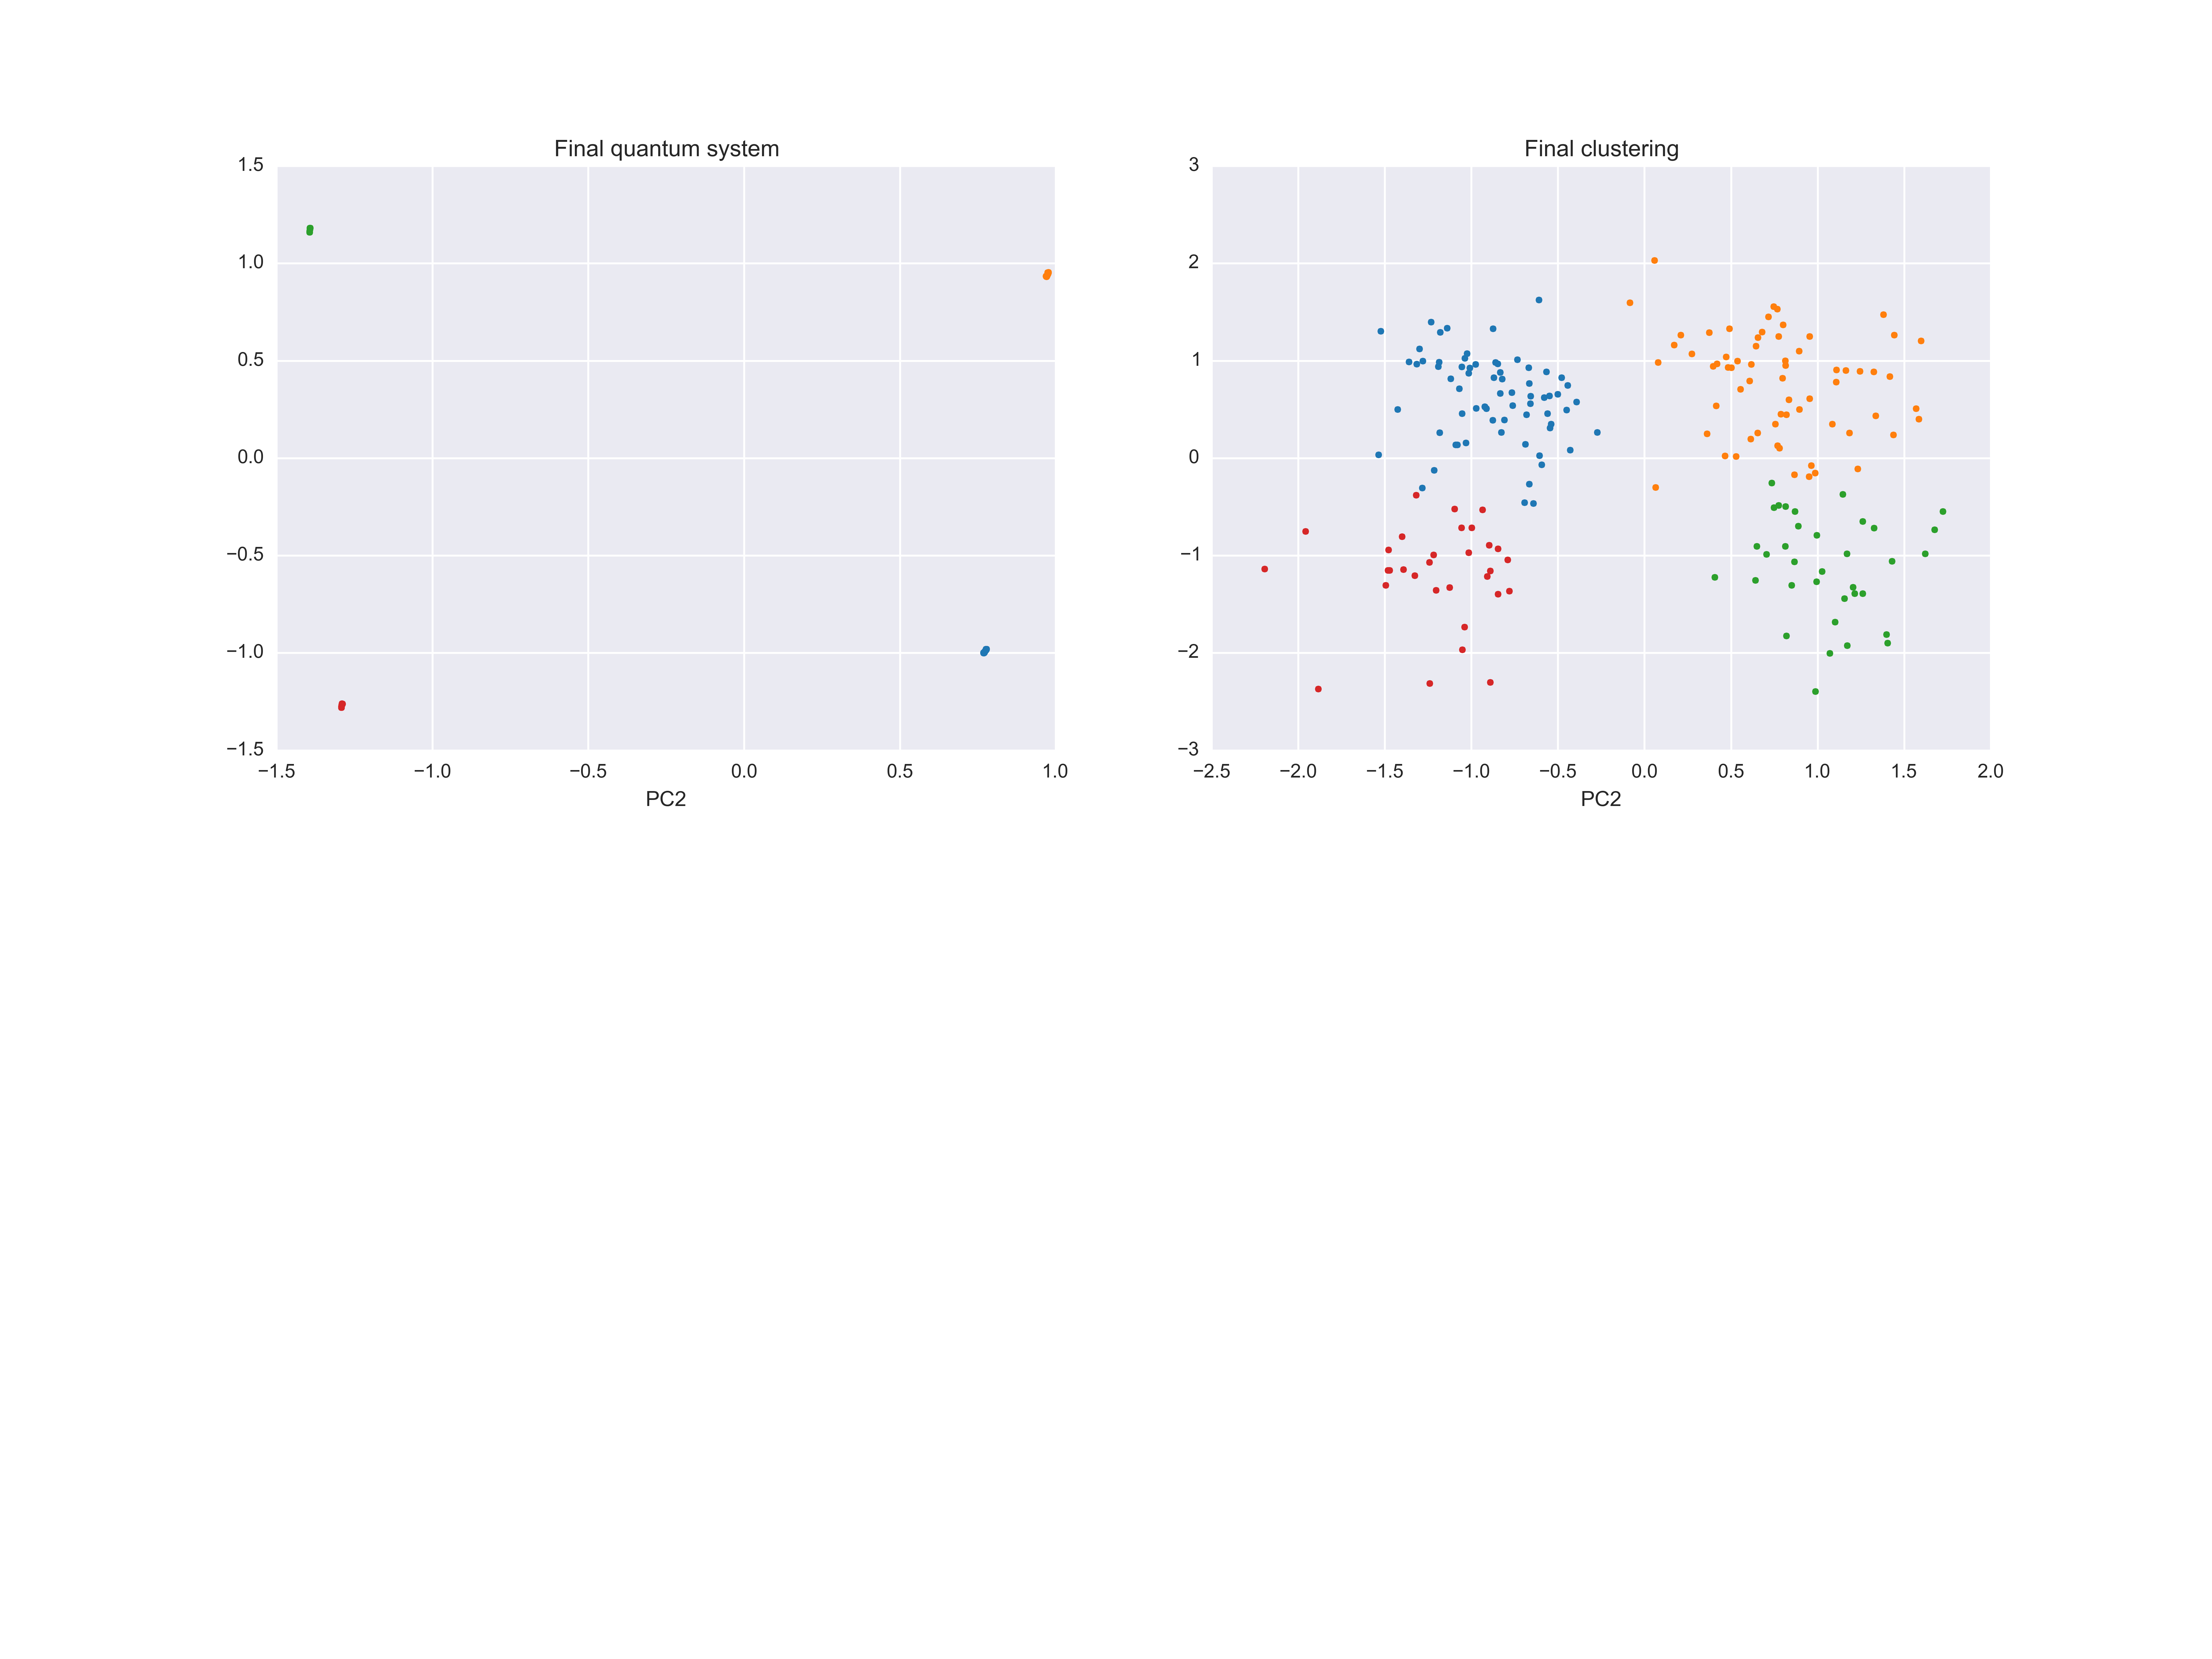
\includegraphics[width=\textwidth]{Horn/img/crab_2pc_covar_cluster.png}
\caption{Representation of the crab data projected over PC 2 and 3.}
\label{fig:crab_2pc_covar_cluster}
\end{figure}

\begin{figure}[hbtp]
\centering
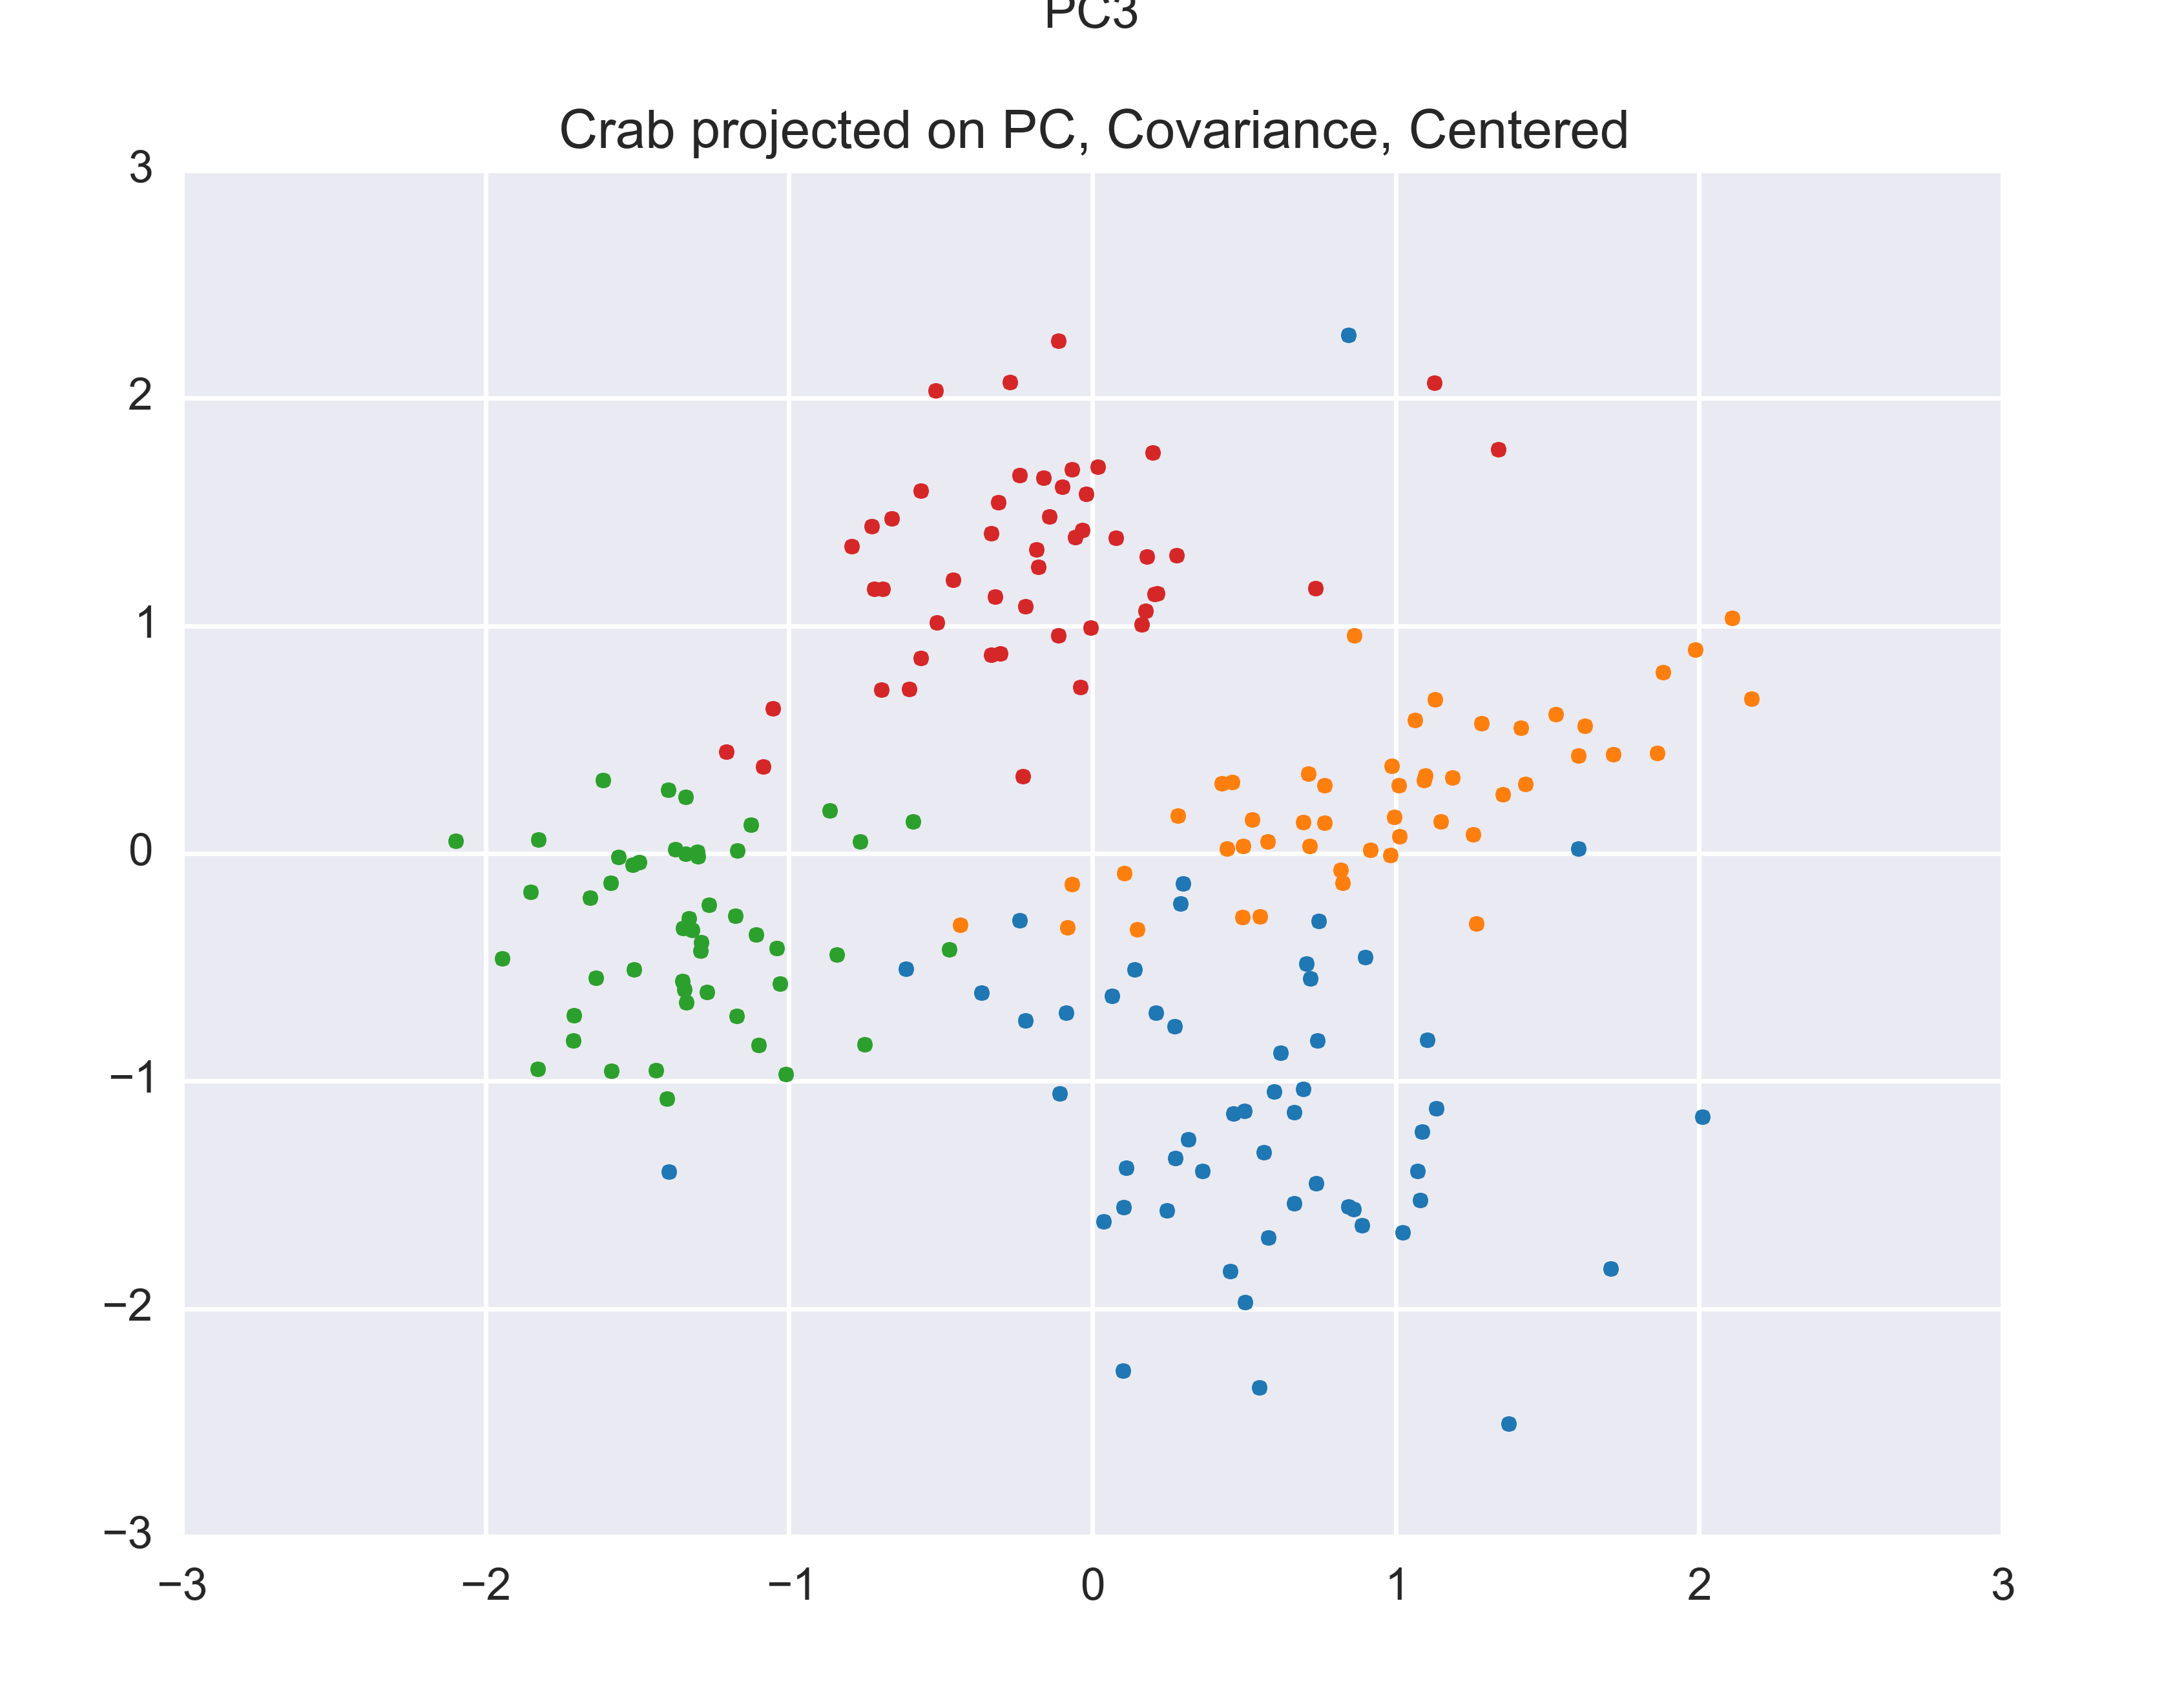
\includegraphics[scale=0.5]{Horn/img/crab_2pc_covar_centered.png}
\caption{Representation of the crab data projected over PC 2 and 3.}
\label{fig:crab_2pc_covar_centered}
\end{figure}

\begin{figure}[hbtp]
\centering
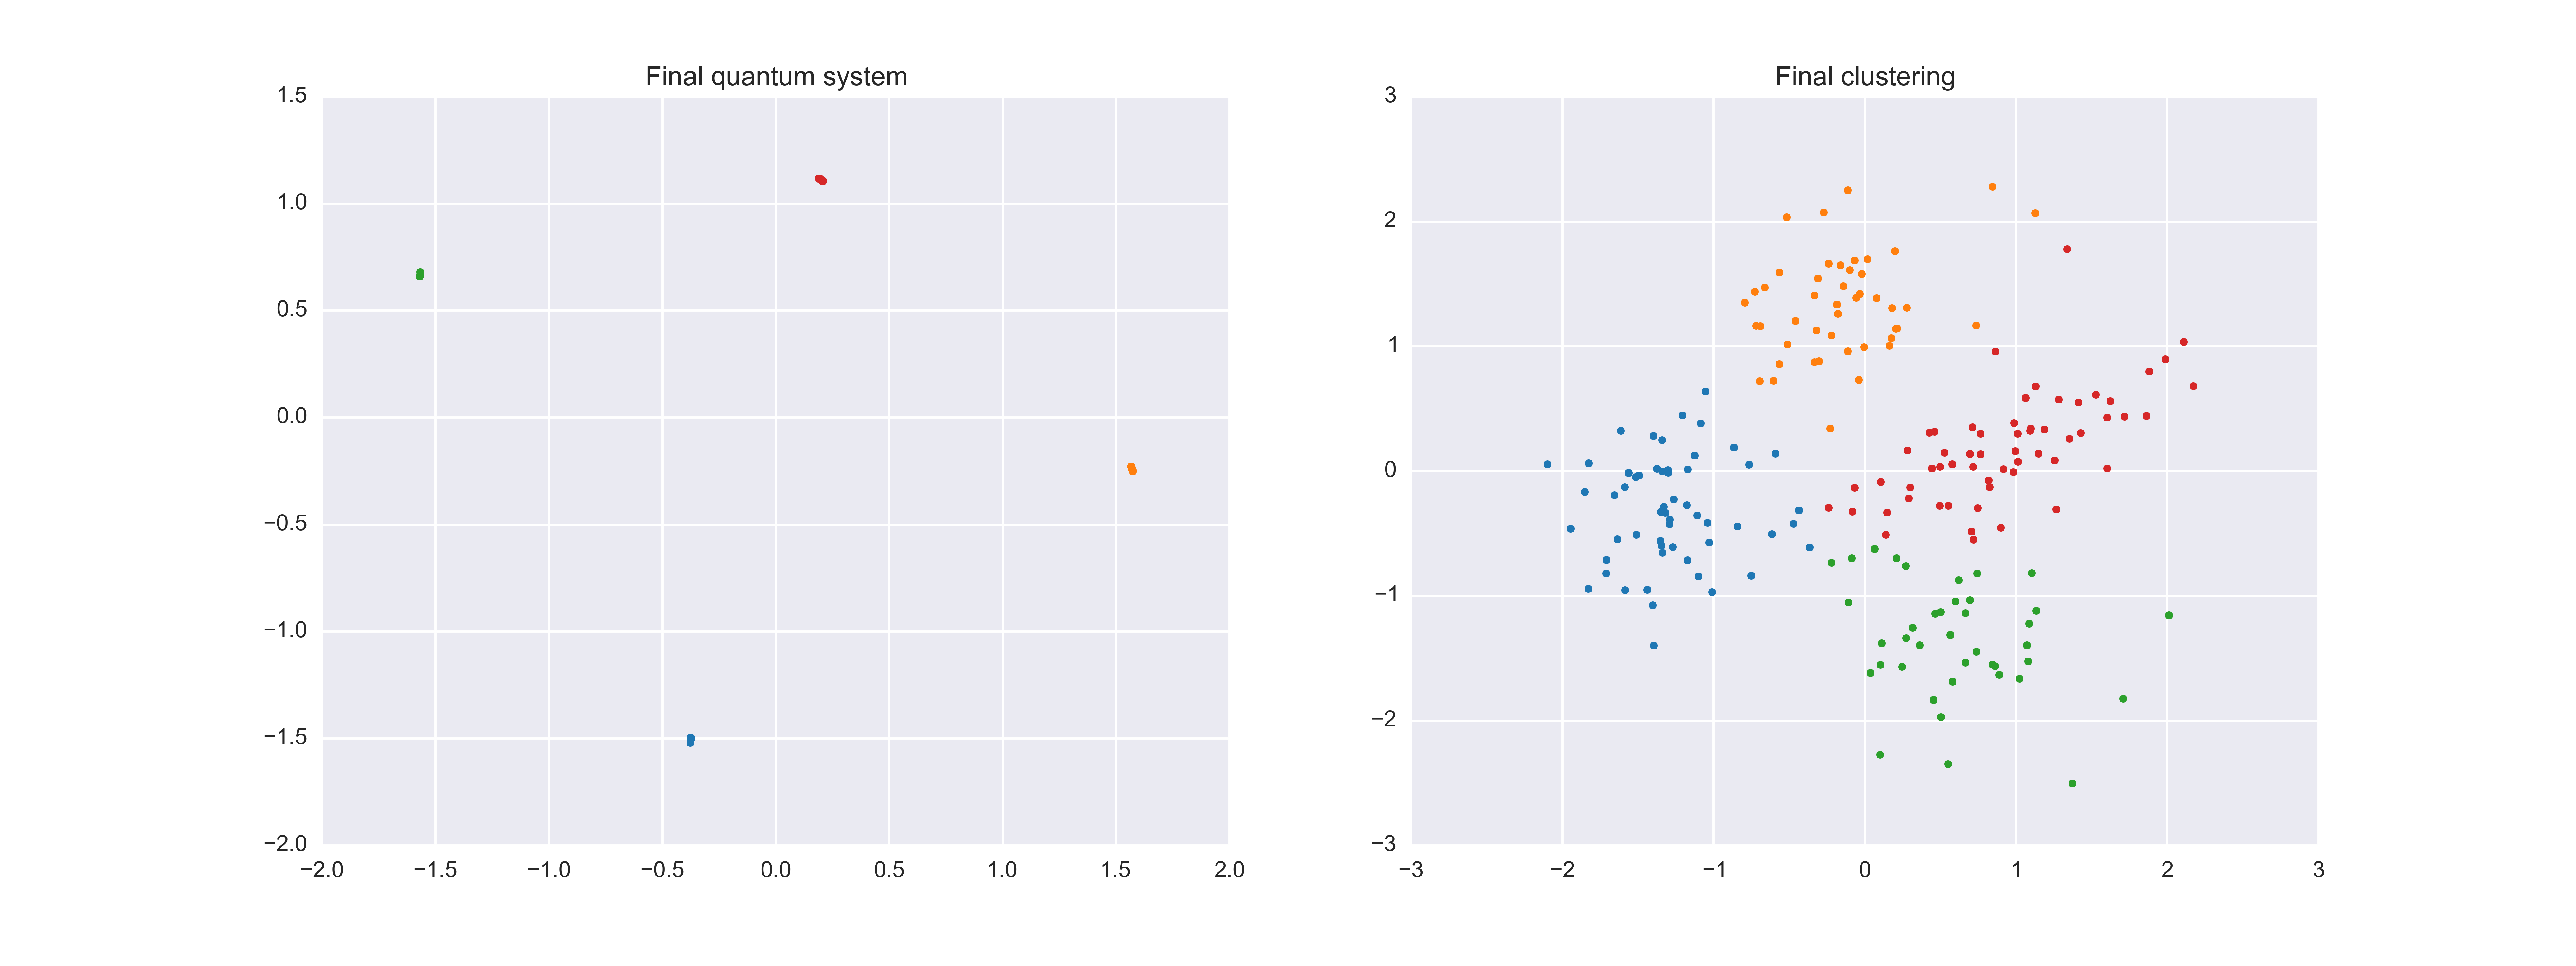
\includegraphics[width=\textwidth]{Horn/img/crab_2pc_covar_centered_cluster.png}
\caption{Representation of the crab data projected over PC 2 and 3.}
\label{fig:crab_2pc_covar_centered_cluster}
\end{figure}


Initial work aimed at reproducing results from [2], but lack of detail on the preprocessing used made it an harder task. Several preprocessings were used, namely whitening or not the data, centring it or not, using covariance versus correlation and different methods of computing the PCs through eigenvalue decomposition or Singular Value Decomposition (SVD). The closest representation to that of the [2] is the one if Fig. C1.


%TODO finish crab

Covariance uncentred consistency index = 0.815
Covariance centred consistency index = 0.91

all pc covariance uncentred consistency index = 0.63
all dimensions original data consistency index = 0.34


\subsection{GPGPU K-Means}




\subsection{K-prototypes influence on coassocs} % file "Thesis_Results.tex"
%!TEX root = Thesis.tex

\chapter{Discussion?}
\label{chapter:discussion}

\section{real num assocs compared to samples per cluster}

\cite{Lourenco2010} reports that, on average, \"the overall contribution of the clustering ensemble (including unbalanced clusters) duplicates the co-associations produced in a single balanced clustering with Kmin clusters\".
However, the spectrum of datasets evaluated regarding cardinality was smaller than that evaluated in the present work.
The results suggest that the contribution of the ensemble is in fact higher. %TODO check if this is true because I only have the data for the maximum number of assocs and not the average one

\section{Trade-off speed accuracy memory}

%TODO
% in the Discussion or Conclusions chapter, include a reflection along the folloing lines
When a problem of clustering of big data is at hand, the user should reflect upon what the problem at hand really requires: speed or accuracy. The user should take into consideration the nature of the data and the requirements of the problem (concerning speed and accuracy) before proceeding to the execution of the analysis. The present body of work reflects a method of clustering over big data using a high accuracy, but also high cost, method. Other methods offer the opposite, low cost, low to average accuracy. 

\section{GPU MST}

The parallel version of the final step of EAC showed a slowdown relative to its sequential counterpart.
This slowdown is related with the performance of the MST algorithm.
The implementation of the algorithm was tested in some of the same graphs as those reported in \cite{Sousa2015} and revealed a speedup.
However, when using the this MST solver on the target graphs (the co-association matrices) not only there was no speedup, but a significantly slowdown was observed, reaching up to nine times slower.
The underlying reason for this is believed to be that the number of edges to node ratio of these graphs is low compared to that typically seen in co-associations matrix, even when using a prototype subset of the original matrix.
Since the parallel computation is anchored to nodes, the workload per node is higher from the beginning and can increase significantly as the algorithm progresses.
Furthermore, the workload can become highly unbalanced with some threads having to process hundreds of thousands of edges while others only a few thousands.


\section{Expanding this work to other scalability paradigms}
% TODO: the idea of this section is to state the main ideas behind the scalability of EAC and see if they are transferable for other scalability paradigms, e.g. clusters
The present work focused on two main approaches for scalability: GPGPU and out-of-core solution. A current trend in computing of big data is cluster computing, which allows for distributed and parallel computing. For the sake of completeness it is interesting to discuss if the ideas related to the former two paradigms are transferable to the later.

The concept of GPGPU is one of parallelization. It is based on the fact that each computing thread in the GPU will execute instructions on a restricted subset of the entire dataset. This idea is easily transferable to cluster computing, as it is a core concept on both paradigms.
For this reason, the generation of the ensemble is a step of EAC that can be very easily transfered to a computing cluster.

%%%%%%%%%%%%%%%%%%%%%%%%%%%%%%%%%%%%%%%%%%%%%%%%%%%%%%%%%%%%%%%%%%%%%%%%
%                                                                      %
%     File: Thesis_Conclusions.tex                                     %
%     Tex Master: Thesis.tex                                           %
%                                                                      %
%     Author: Andre C. Marta                                           %
%     Last modified : 21 Jan 2011                                      %
%                                                                      %
%%%%%%%%%%%%%%%%%%%%%%%%%%%%%%%%%%%%%%%%%%%%%%%%%%%%%%%%%%%%%%%%%%%%%%%%

\chapter{Conclusions}
\label{chapter:conclusions}

Insert your chapter material here...


% ----------------------------------------------------------------------
\section{Achievements}
\label{section:achievements}

The major achievements of the present work...


% ----------------------------------------------------------------------
\section{Future Work}
\label{section:future}

%further optimization on K-Means
% using local memory to speed-up
% study on optimal number of pointer per thread

% other algorithms in the first and last phase
Much effort was put developing and testing co-association matrix building strategies.
The schemes presented here provide a solid framework to work with large data sets in this middle step of EAC.
As such, interesting directions for this work to take are testing how state of the art algorithms designed for Big Data would complement EAC in the first and last steps.

The programming model used for the GPU was CUDA, used through a Python library called Numba.
This library offers an interface to access most of CUDA's capabilities, but not all.
One of those capabilities is Dynamic Parallelism.
This offers the ability of having a host kernel call on other host kernel without intervention from the host.
This translates in the possibility of moving the control logic in the Borůvka variant (and also its the Connected Components Labeling variant) to the device, effectevely removing the memory transfer of values related with the control logic.

Adaptation of the present implementation to OpenCL. This brings major benefits in respect to portability since OpenCL supports most devices. Moreover, OpenCL's performance is catching in on that of CUDA's and since it's programming model was based on CUDA, it should be straightforward for developers to make the switch.

Application of EAC to the MapReduce framework will further expand the possibilities of application of EAC.

Study the integration of other clustering algorithms within the the EAC toolchain.

A good follow-up of the present work is to study the relationship between several metrics (e.g. sparsity, accuracy, maximum number of co-associations) and the complexity of the dataset. Some metrics for describing the complexity of the dataset exist (Tin Kam Ho) and it would be interesting to profile several datasets of different complexities and structures and search for the former relationship.
On a performance perspective it could prove useful to deduce better rules to set the maximum number of associations in the sparse matrix.
On a accuracy perspective it would be interesting to see if there are types of datasets that simply are not a good fit for EAC while other are. It would also be interesting to relate complexity with the threshold cut-off.

% cross with WEAC
The WEAC algorithm is focused on improving accuracy.
The underlying concept is to measure the quality of the partitions in the ensemble and allow the better ones to be more influential in the co-association matrix.
The concept of measuring the quality of the partitions may prove useful for further decreasing the memory complexity with the EAC CSR scheme without compromising too much accuracy.
The basic idea is to choose a $max\_assocs$ value that will likely be less than the number of associations many patterns will have, which will result in some associations being discarded.
The associations that will be kept are the ones from the first partitions that were processed.
With this in mind, one could order the partitions by quality and start the processing from those with better quality.

% More efficient external sorting
% It is believed that a significant speedup may be obtained by using GPUs for external sorting in the argsort step of the cluster recovery of EAC.
% Even without using GPU's further speedup may be possible simply by using more memory. After the co-association matrix is stored it can be deleted from main memory. This means that almostthe entire memory is available for the computation of the argsort array. Currently the PyTables CSI algorithm uses a insignificant amount of memory.

\cleardoublepage

 % file "Thesis_Conclusions.tex"

% ----------------------------------------------------------------------
%  Bibliography
% ----------------------------------------------------------------------

% Include all references in .bib file, even non-cited ones...
%\nocite{*} % this should be used carefully because it is not correct!

% Produces the bibliography section when processed by BibTeX
%
% Bibliography style
% > entries ordered alphabetically
%\bibliographystyle{plain}
% > unsorted with entries appearing in the order in which the citations appear.
%\bibliographystyle{unsrt}
% > entries ordered alphabetically, with first names and names of journals and months abbreviated
%\bibliographystyle{abbrv}
% > entries ordered alphabetically, with reference markers based on authors' initials and publication year
%\bibliographystyle{alpha}
%
% Replacement bibliography styles provided by 'natbib' package
% (plainnat.bst, abbrvnat.bst, unsrtnat.bst )
% > entries ordered alphabetically
%\bibliographystyle{plainnat}
% > unsorted with entries appearing in the order in which the citations appear.
\bibliographystyle{unsrtnat}
% > entries ordered alphabetically, with first names and names of journals and months abbreviated
% \bibliographystyle{abbrvnat}
% > entries ordered alphabetically, with reference markers based on authors' initials and publication year
%\bibliographystyle{alpha}


% External bibliography database file in the BibTeX format
\cleardoublepage
\bibliography{library} % file "Thesis_bib_DB.bib"
% Add entry in the table of contents as chapter
\addcontentsline{toc}{chapter}{\bibname}
\cleardoublepage

% ----------------------------------------------------------------------
%  Appendix (optional)
% ----------------------------------------------------------------------
\appendix
%%%%%%%%%%%%%%%%%%%%%%%%%%%%%%%%%%%%%%%%%%%%%%%%%%%%%%%%%%%%%%%%%%%%%%%%
%                                                                      %
%     File: Thesis_Appendix.tex                                        %
%     Tex Master: Thesis.tex                                           %
%                                                                      %
%     Author: Andre C. Marta                                           %
%     Last modified : 21 Jan 2011                                      %
%                                                                      %
%%%%%%%%%%%%%%%%%%%%%%%%%%%%%%%%%%%%%%%%%%%%%%%%%%%%%%%%%%%%%%%%%%%%%%%%

\chapter{Vector calculus}
\label{chapter:appendixVectors}

In case an appendix if deemed necessary, the document cannot exceed a total of 100 pages...

Some definitions and vector identities are listed in the section below.

% ----------------------------------------------------------------------
\section{Vector identities}
\label{section:vectorIdentities}

\begin{equation}
	\nabla \times \left( \nabla \phi \right) = 0
	\label{eq:cross_nnp}
\end{equation}

\begin{equation}
	\nabla \cdot \left( \nabla \times {\bf u} \right) = 0
	\label{eq:dotCross_nnu}
\end{equation}

\cleardoublepage

 % file "Thesis_Appendix.tex"

% ----------------------------------------------------------------------
\end{document}
% ----------------------------------------------------------------------

